\chapter[Optical Phenomena; Properties of Matter]{Optical Phenomena and Properties of Matter}
\label{p:mm:op12}


%\begin{pspicture}
%\psspectrum[absorption,lines={400,434.8,476.2,526.3,588.2,666.7},lwidth=0.1](\linewidth,1)
%\end{pspicture}
%\psspectrum[element={Hg,Cd2+,W+}]
%\psspectrum[element=F](\linewidth,1)

\section {Introduction}
For centuries physicists argued about whether light was a particle or a wave. It was assumed that light could only be one or the other, but not both.
 
%In earlier chapters on waves (Chapters~\ref{p:wsl:tw10}, \ref{p:wsl:de12}, \ref{p:wsl:c12}, \ref{p:wsl:2d3d12}) and optics (Chapters~\ref{p:wsl:go10} and \ref{p:wsl:go11}), you studied how light or other electromagnetic radiation propagates like a wave. The wave nature of light was demonstrated by the propagation of light in examples such as diffraction, interference, and polarisation of light.

In earlier chapters on waves and optics, you studied how light or other electromagnetic radiation propagates like a wave. The wave nature of light was demonstrated by the propagation of light in examples such as diffraction, interference, and polarisation of light.

 
You also saw in Electromagnetic Radiation how light sometimes behaves as a particle. This chapter looks at evidence supporting the \textit{particle model of light}. The idea that light can have both wave and particle properties was one of the most important discoveries of the twentieth century.

\chapterstartvideo{VPpxi}

\section{The transmission and scattering of light}
%\begin{syllabus}
%\item Learners must be able to explain the interaction of uv and visible radiation with metals (reflection by absorbtion and and re-emission) in terms of the interaction with electromagnetic radiation
%\item Explain why the sky is blue
%\item Notes: Link the interaction of matter with light to the electronic properties of matter (grade 11 electrical conduction)
%\end{syllabus}

\subsection{Energy levels of an electron}
We have seen that the electrons in an atom have different energy levels. When the electron receives enough energy, it can jump up to a higher energy level. This is called \textit{'exciting'} the electron. When the electron in a high energy level sheds some energy, it drops to a lower energy level. 
 
We have also seen that the energy associated with light at a specific wavelength is given by:
\nequ{E=\frac{h c}{\lambda}.}
 In the particle model of light, this means that each packet of light (photon) at a wavelength $\lambda$ has energy:
\nequ{E=\frac{h c}{\lambda}.}

For the electron to receive energy, it \textit{absorbs} a photon and gets its energy. When an electron loses energy to drop to a lower level, it \textit{emits} (gives off) a photon with that energy. 

\subsection{Interaction of light with metals}
When light encounters or passes through a material, the photons of the light interact with the atoms or molecules of the material.  Depending on the strength of the interactions and how often they happen, the light will pass through the material or be scattered in some other direction.
 
Each wavelength of light relates to a particular energy, and the closer that energy is to the energy difference between two of the levels of the atom, the likelier the photon is to interact with the atom.
 
When visible or ultraviolet (UV) radiation shines on a metal, the photons are \textit{absorbed} by the electrons in the metal. The electrons are then excited up to a higher energy level. When an electron returns to a lower energy level, another photon is emitted. This is how light appears to be \textbf{reflected} off a metal surface. 
 
In previous chapters, you have studied geometrical optics, which tells us what happens to rays of light when they are reflected off a surface or refracted through a lens.  That tells us what happens to light rays, made up of many photons, on a large scale.  If you look at a smaller level, i.e.\@ on a microscopic scale, then reflection and refraction happen by all the photons interacting with the atoms of the lens or mirror.  The photons get absorbed and re-emitted many times before emerging as the finals rays of light that we see.
 
%The dependence of the scattering of light on the energy levels of the materials it encounters is responsible for many effects that we see in %everyday life.  
Scattering of light is responsible for many effects in everyday life.
We see that certain materials are red or blue, for example, since they contain materials that have energy level differences that correspond to the energies of the photons that make up red or blue light.  These materials then reflect the red or blue light and absorb the other wavelengths in the visible spectrum.  White objects reflect photons of all wavelengths in the visual spectrum, while black objects absorb these photons.

\begin{IFact}{Because a truly black object absorbs all the visual wavelengths of light, and does not re-emit photons at visual wavelengths, we can say that 'black' is not a colour itself, but rather a \textit{lack of} colour! Also, since black objects absorb visual light, they heat up more than objects of other colours which reflect light at certain wavelengths.}
\end{IFact}

\Activity{Investigation}{Reflection and absorption}
{
\Aim{Investigate the interaction of light with differently coloured metal objects}
\Apparatus{Find some differently coloured metal objects (at least 5) which will not be damaged if left in the sun for 15 minutes. Make sure to include at least one white item and one black item.}
\Method{At the start of your lesson set out your objects in direct sunlight. Leave them there for around 15 minutes.

Alternatively, if it is a sunny day, you can use your teachers' cars for this experiment - as long as there are some cars of different colours and they have been standing in direct sunlight for the same length of time! } 

After 15 minutes is up, touch each of the items/cars (be careful not to burn yourself!) and compare their temperatures (rate them from 1 to 5 with 1 being cold and 5 being very hot) in a table such as the example table below:

\begin{center}
\begin{tabular}{ | c | c | c |}
\hline
\textbf{Object} & \textbf{Colour} & \textbf{Temperature rating} \\ \hline \hline
e.g.\@ car 1 & e.g.\@ red & e.g.\@ 3 \\ \hline
   &      &    \\
\hline
\end{tabular}
\end{center}

\textbf{Questions:}\\
\begin{enumerate}
\item Which object was the hottest and what was it made of?
\item Which object was the coolest and what was it made of?
\item How did the temperatures of the black and white objects compare to each other? (which one was hotter and which was cooler?)
\item Try to explain the reasons for the different temperatures of the objects with respect to their colours and the materials of which they are made. 
\end{enumerate}
}
 
Metals generally reflect most wavelengths of visible light, but they will reflect the light in a certain direction, given by the laws of reflection in geometrical optics.  This is different to most materials, like wood or fabric, which reflect light in all directions.  Metals have this property since they have electrons that are not bound to atoms and can move freely through the metal. This is unlike most other materials that have their electrons bound closely to the atoms.  These free electrons in metals can then absorb and reflect photons of a wide range of energies. 

\textit{Ultraviolet light} (which has shorter wavelengths than visible light) will pass through some substances, such as many plastics, because they do not have the right energy levels to absorb it and re-emit it. \textit{X-rays} (also short wavelengths) will also pass through most materials, since the energies of X-rays correspond to the energy levels of atomic nuclei.  Such nuclei are much smaller than atoms, so it is much less likely for an X-ray to hit a nucleus instead of the whole atom.

Most materials will absorb \textit{infrared radiation} (longer wavelengths than visible light), since the energies of that radiation often correspond to rotational or vibrational energy levels of molecules. 

\begin{figure}[!tb]
\begin{center}
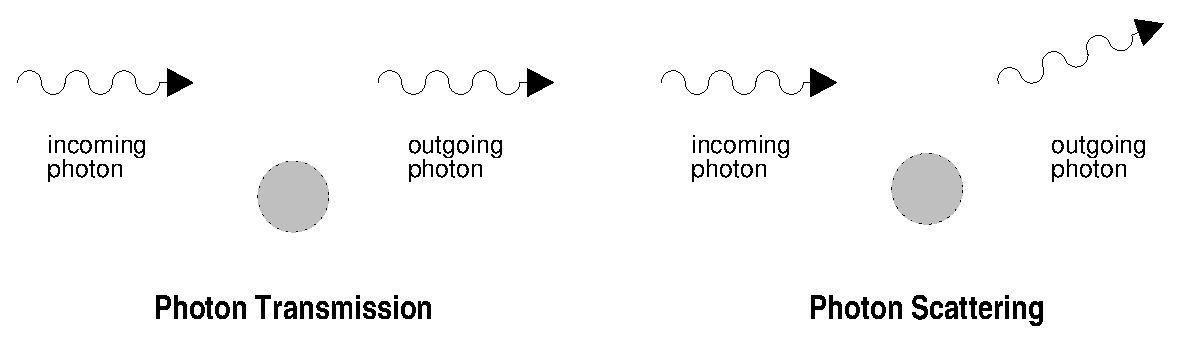
\includegraphics[width=4.5in]{../../epsimages/photon_scatter_transmission.eps}
\end{center}
\caption{Diagrams of photon transmission (left) and scattering (right).}
\label{transscatter}
\end{figure}

 
\subsection{Why is the sky blue?}
The sun emits light at many different wavelengths, including all of the visible wavelengths. Light which is made up of all the visible wavelengths appears white. So what causes the sky to look blue?

The atmosphere consists of molecules of different gases as well as tiny dust grains. Light from the sun scatters off the molecules in the air (called \textbf{Rayleigh scattering}).  
The chance that the light will scatter off the gas molecules is \textit{higher} for \textit{shorter} wavelengths.  The \textit{short wavelength} \textbf{blue light} is therefore scattered more than the other colours.  At noon, when the light from the sun is coming straight down (see the picture), the scattered blue light reaches your eyes from all directions and so the sky appears blue. The other wavelengths do not get scattered much and therefore miss your line of sight and are not seen. At sunrise or sunset, the direction of the light coming from the sun is now straight towards your eyes (see the picture). Therefore the scattered blue light can't be seen because it is scattered out of your line of sight. The redder colours (oranges and reds) can now be seen because they are not scattered as much and still fall in your line of sight. 
 


\begin{center}
\scalebox{1} % Change this value to rescale the drawing.
{
\begin{pspicture}(0,-2.38)(7.8,2.38)
\definecolor{color1652}{rgb}{0.6,0.6,0.6}
\psbezier[linewidth=0.04](1.34,-2.34)(1.76,-1.92)(5.06,-1.62)(6.04,-2.36)
\psbezier[linewidth=0.04](2.96,2.34)(3.04,1.66)(4.76,1.56)(4.88,2.36)
\psline[linewidth=0.04cm](2.98,2.04)(2.58,1.7)
\psline[linewidth=0.04cm](3.3,1.8)(3.02,1.4)
\psline[linewidth=0.04cm](3.66,1.74)(3.6,1.28)
\psline[linewidth=0.04cm](4.04,1.74)(4.1,1.24)
\psline[linewidth=0.04cm](4.42,1.8)(4.6,1.38)
\psline[linewidth=0.04cm](4.8,2.02)(5.18,1.6)
\psellipse[linewidth=0.04,dimen=outer](3.59,-1.14)(0.11,0.16)
\psline[linewidth=0.04cm](3.58,-1.28)(3.58,-1.68)
\psline[linewidth=0.04cm](3.58,-1.66)(3.72,-1.88)
\psline[linewidth=0.04cm](3.58,-1.68)(3.42,-1.88)
\psline[linewidth=0.04](3.44,-1.4)(3.58,-1.58)(3.72,-1.42)
\psbezier[linewidth=0.04,arrowsize=0.05291667cm 2.0,arrowlength=1.4,arrowinset=0.4]{->}(4.129678,1.802414)(4.0782003,1.7414411)(4.364416,1.3757231)(4.210351,1.3212587)(4.056286,1.2667943)(4.120731,0.99075055)(4.2747455,1.0081792)(4.42876,1.0256077)(4.4956264,0.6901674)(4.337112,0.66049534)(4.1785975,0.63082325)(4.251798,0.31939214)(4.4103127,0.34906423)(4.568827,0.3787363)(4.64,0.032700967)(4.4814854,0.003028889)(4.322971,-0.026643187)(4.496376,0.10848992)(4.567576,-0.46)
\psline[linewidth=0.05cm,linecolor=color1652,linestyle=dashed,dash=0.16cm 0.16cm](4.58,-0.46)(4.9,-1.86)
\psbezier[linewidth=0.04,arrowsize=0.05291667cm 3.0,arrowlength=1.4,arrowinset=0.4]{->}(4.54,-0.40787914)(4.4937525,-0.44371104)(4.4733295,-0.54631287)(4.441706,-0.4994201)(4.4100833,-0.45252737)(4.347896,-0.49794462)(4.3865466,-0.555258)(4.425197,-0.61257136)(4.366038,-0.6691876)(4.3282733,-0.61122465)(4.2905087,-0.55326164)(4.230578,-0.6134802)(4.2680573,-0.66905683)(4.3055367,-0.7246334)(4.2472634,-0.7806001)(4.2117267,-0.72315794)(4.1761894,-0.66571575)(4.1116886,-0.72194)(4.1515107,-0.7809901)(4.1913323,-0.84004027)(4.131117,-0.89787245)(4.0951796,-0.83509123)(4.0592427,-0.77230996)(4.000198,-0.83187896)(4.0369062,-0.89105785)(4.0736146,-0.95023674)(4.015341,-1.0062034)(3.9774616,-0.9452877)(3.939582,-0.88437206)(3.8797662,-0.9475433)(3.918417,-1.0048567)(3.9570677,-1.06217)(3.9199593,-0.99765205)(3.8193521,-1.1)
\psbezier[linewidth=0.04,arrowsize=0.05291667cm 2.0,arrowlength=1.4,arrowinset=0.4]{->}(4.563167,-0.42788064)(4.554229,-0.46518552)(4.770936,-0.6485422)(4.7138457,-0.68920416)(4.656756,-0.7298661)(4.7514534,-0.87855685)(4.817297,-0.85843486)(4.883141,-0.8383128)(4.993015,-1.0197747)(4.9280276,-1.0469913)(4.863041,-1.0742079)(4.970103,-1.2419266)(5.0350895,-1.21471)(5.100076,-1.1874933)(5.2144175,-1.3745377)(5.1494303,-1.4017544)(5.0844436,-1.428971)(5.131203,-1.342265)(5.2982745,-1.652659)
\rput(1.82,1.105){At noon, sun is overhead}
\rput(5.7,0.78){\footnotesize sun emits radiation}
\rput(5.69,0.48){\footnotesize of all wavelengths}
\rput(3.14,-0.3){\footnotesize blue light scattered}
\rput(2.85,-0.56){\footnotesize by large angle}
\rput(2.69,-0.86){\footnotesize into the eye}
\rput(6.34,-0.66){\footnotesize red light scattered little}
\rput(6.15,-0.94){\footnotesize and misses the eye}
\end{pspicture} 
}
\end{center}

\begin{center}
\scalebox{1} % Change this value to rescale the drawing.
{
\begin{pspicture}(0,-1.96)(8.5465355,1.98)
\definecolor{color1960}{rgb}{0.6,0.6,0.6}
\psbezier[linewidth=0.04](1.24,-1.7)(1.66,-1.28)(4.96,-0.98)(5.94,-1.72)
\psbezier[linewidth=0.04](8.513465,0.21002984)(7.8331804,0.1324845)(7.7269735,-1.5871434)(8.526535,-1.7100298)
\psline[linewidth=0.04cm](8.22,0.12)(7.8,0.62)
\psline[linewidth=0.04cm](8.010457,-0.21053997)(7.4895434,0.09053997)
\psline[linewidth=0.04cm](7.92,-0.5)(7.32,-0.4)
\psline[linewidth=0.04cm](7.9,-0.86)(7.32,-0.96)
\psline[linewidth=0.04cm](8.02,-1.3)(7.52,-1.52)
\psline[linewidth=0.04cm](8.18,-1.62)(7.82,-1.94)
\psellipse[linewidth=0.04,dimen=outer](3.81,-0.52)(0.11,0.16)
\psline[linewidth=0.04cm](3.8,-0.66)(3.8,-1.06)
\psline[linewidth=0.04cm](3.8,-1.04)(3.94,-1.26)
\psline[linewidth=0.04cm](3.8,-1.06)(3.64,-1.26)
\psline[linewidth=0.04](3.66,-0.78)(3.8,-0.96)(3.94,-0.8)
\psbezier[linewidth=0.04,arrowsize=0.05291667cm 2.0,arrowlength=1.4,arrowinset=0.4]{->}(7.9119506,-0.8102876)(7.8759775,-0.73905927)(7.4274335,-0.85938114)(7.4375854,-0.696288)(7.447737,-0.5331948)(7.1684833,-0.48450622)(7.124267,-0.6330632)(7.0800514,-0.7816202)(6.745188,-0.7119222)(6.7798967,-0.5544338)(6.8146057,-0.39694548)(6.4993596,-0.34247005)(6.4646506,-0.49995843)(6.4299417,-0.6574468)(6.083643,-0.5875668)(6.118352,-0.43007845)(6.153061,-0.27259007)(6.2095814,-0.48504156)(5.658549,-0.32815576)
\psline[linewidth=0.05cm,linecolor=color1960,linestyle=dashed,dash=0.16cm 0.16cm](5.653688,-0.33958933)(4.2400846,-0.08635944)
\psbezier[linewidth=0.04,arrowsize=0.05291667cm 3.0,arrowlength=1.4,arrowinset=0.4]{->}(5.7173038,-0.32316893)(5.702421,-0.26658913)(5.615988,-0.20765318)(5.6715145,-0.19689642)(5.7270417,-0.18613966)(5.709574,-0.11114067)(5.641708,-0.12428783)(5.5738416,-0.13743499)(5.544883,-0.060840968)(5.6130004,-0.048763357)(5.681118,-0.036685742)(5.649146,0.042027358)(5.5833364,0.0292786)(5.5175266,0.016529841)(5.488819,0.092054315)(5.555586,0.102285594)(5.6223526,0.112516865)(5.5958447,0.1938731)(5.525922,0.18032755)(5.4559984,0.16678199)(5.4263344,0.24482395)(5.4981713,0.25333455)(5.570008,0.26184514)(5.538287,0.3394887)(5.469464,0.328859)(5.4006405,0.31822935)(5.3719335,0.3937538)(5.442813,0.40478188)(5.513693,0.41580996)(5.4789586,0.4955726)(5.4110923,0.48242545)(5.343226,0.46927828)(5.4171195,0.47818726)(5.36229,0.610817)
\psbezier[linewidth=0.04,arrowsize=0.05291667cm 2.0,arrowlength=1.4,arrowinset=0.4]{->}(5.6898327,-0.33666438)(5.658998,-0.31384376)(5.405474,-0.44154257)(5.3903885,-0.37309492)(5.375303,-0.30464724)(5.2014155,-0.33362415)(5.1941733,-0.4020921)(5.1869316,-0.47056004)(4.9769473,-0.50068235)(4.977325,-0.43022746)(4.9777026,-0.35977256)(4.7814665,-0.3926839)(4.781089,-0.4631388)(4.780711,-0.5335937)(4.563842,-0.5656432)(4.5642195,-0.49518833)(4.564597,-0.42473343)(4.6260986,-0.50168794)(4.2750816,-0.53400683)
\rput(2.54,1.785){At sunrise/sunset, sun is at horizon}
\rput(6.3,1.36){\footnotesize blue light scattered}
\rput(6.03,1.06){\footnotesize by large angle}
\rput(6.31,0.74){\footnotesize away from the eye}
\rput(5.25,-0.76){\footnotesize red light scattered}
\rput(4.89,-1.04){\footnotesize into the eye}
\end{pspicture} 
}
\end{center}

\Exercise{Transmission and scattering of light}{
\begin{enumerate}
\item{Explain how visible light is reflected from metals.}
\item{Explain why the sky is blue.}
\end{enumerate}

% Automatically inserted shortcodes - number to insert 2
\par \practiceinfo
\par \begin{tabular}[h]{cccccc}
% Question 1
(1.)	01mn	&
% Question 2
(2.)	01mp	&
\end{tabular}
% Automatically inserted shortcodes - number inserted 2
}

\section{The photoelectric effect}

Around the turn of the twentieth century, it was observed by a number of physicists (including Hertz, Thomson and Von Lenard) that when light was shone on a metal, electrons were emitted by the metal. This is called the photoelectric effect. (\textit{photo}- for light, \textit{electric}- for the electron.)

\Definition{The photoelectric effect}{The photoelectric effect is the process whereby an electron is emitted by a metal when light shines on it.}


At that time, light was thought to be purely a wave. Therefore, physicists thought that if a more intense (i.e.\@ brighter) light was shone on a metal, then the electrons would be knocked out with greater kinetic energies than if a faint light was shone on them. However, Von Lenard observed that this did not happen at all. The \textit{intensity} of the light made \textit{no difference} to the kinetic energy of the emitted electrons! Also, it was observed that the electrons were emitted immediately when light was shone on the metal - there was no time delay.

Einstein solved this problem by proposing that light is made up of packets of energy called \textit{quanta} (now called photons) which interacted with the electrons in the metal like particles instead of waves. Each incident photon would transfer all its energy to one electron in the metal. For a specific colour of light (i.e.\@ a certain wavelength or frequency), the energy of the photons is given by $E = hf = hc/\lambda$, where $h$ is Planck's constant. The energy needed to knock an electron out of the metal is called the \textbf{work function} (symbol $\phi$) of the metal. Therefore, the amount of energy left over as the kinetic energy ($E_{k}$) of the emitted electron would be the difference between the incoming photon's energy and the energy needed to knock out the electron (work function of the metal): 

\begin{eqnarray*}
E_{k} &=& hf - \phi 
\end{eqnarray*} 

Increasing the intensity of the light (i.e.\@ making it brighter) did not change the wavelength of the light and therefore the electrons would be emitted with \textit{the same} kinetic energy as before! This solved the paradox and showed that light has \textit{both} a \textbf{wave nature} and a \textbf{particle nature}. Einstein won the Nobel Prize for this quantum theory and his explanation of the photoelectric effect. 

Increasing the intensity of the light actually means increasing the \textit{number} of incident photons. Therefore, since each photon only gives energy to one electron, more incident photons means \textit{more} electrons would be knocked out of the metal, but their kinetic energies would be \textit{the same} as before. 

\begin{figure}[!h]
\begin{center}
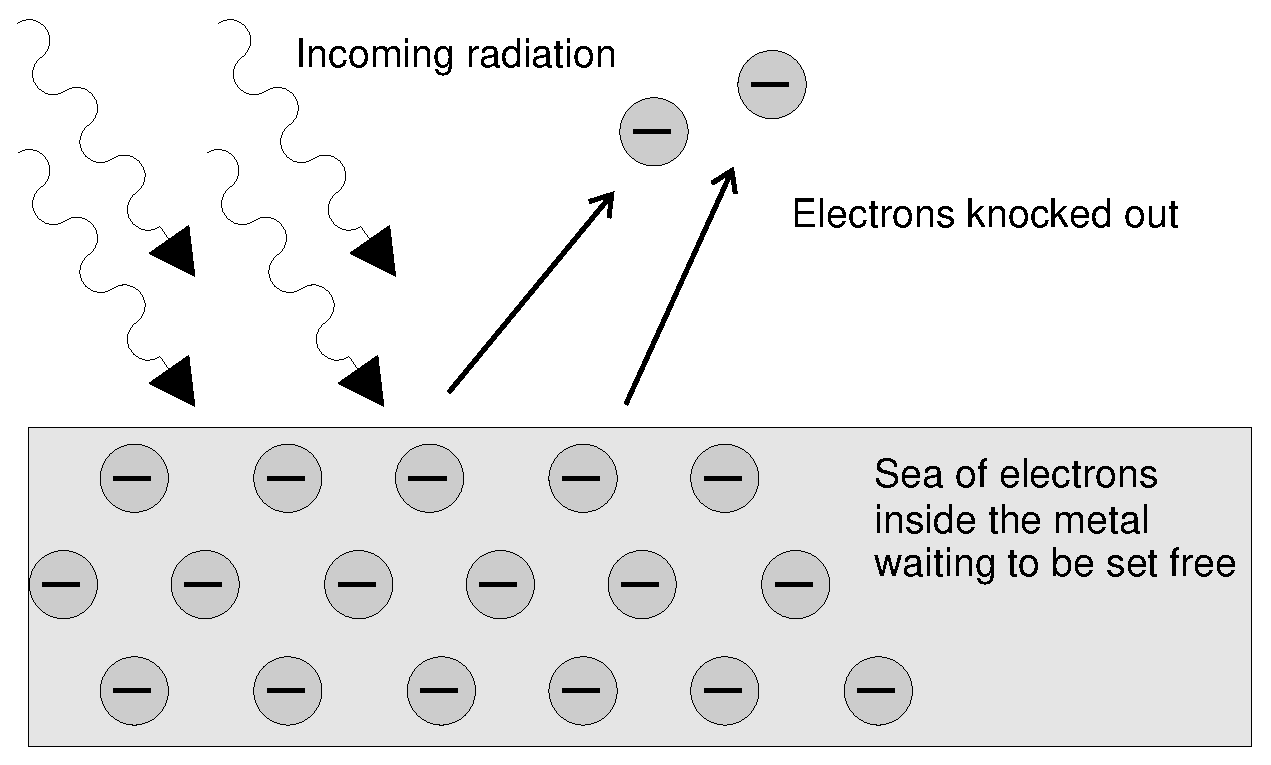
\includegraphics[width=0.5\textwidth]{../../epsimages/Photoelectric_effect.eps}
\caption{The photoelectric effect: Incoming photons on the left hit the electrons inside the metal surface. The electrons absorb the energy from the photons, and are ejected from the metal surface.}
\label{phot_el}
\end{center}
\end{figure}

\begin{IFact}
{The photoelectric effect was first observed in the experiments of Heinrich Hertz in 1887. In 1899 J.J. Thomson proved that it was electrons that were emitted. The photoelectric effect was theoretically explained by Albert Einstein in 1905.}
\end{IFact}
% PhET simulation on the photoelectric effect: SIYAVULA-SIMULATION:http://cnx.org/content/m39551/latest/#id63458

\simulation{Photoelectric effect}{VPpyy}
 
The discovery and understanding of the photoelectric effect was one of the major breakthroughs in science in the twentieth century as it provided concrete evidence of the particle nature of light. It overturned previously held views that light was composed purely of a continuous transverse wave. On the one hand, the wave nature is a good description of phenomena such as diffraction and interference for light, and on the other hand, the photoelectric effect demonstrates the particle nature of light. This is now known as the `dual-nature' of light. (dual means two)

%The new picture considered light (or in general, electromagnetic radiation) to be composed of several 'packets' or 'quanta' (plural for %'quantum') of energy. Each individual photon had a fixed amount of energy depending on the frequency of the electromagnetic radiation.
%However, the wave nature of electromagnetic radiation was also valid since phenomena such as diffraction and interference could only be %explained using the wave nature as they are basic wave properties. Hence a general agreement was reached that light (all electromagnetic %radiations) exhibits a dual nature. Light behave as waves in some cases and behaves as particles in other cases. This came to be known as the %'dual-nature of light'. This  dual-nature of light and all other electromagnetic radiations forms the backbone of quantum mechanics . Note that %the energy of quanta is quantised ($E = hf$) which means that the energy can have a value only in multiples of $h$ (Planck's constant). 
 
While solving problems we need to decide for ourselves whether we should consider the wave property or the particle property of light. For example, when dealing with interference and diffraction, light should be treated as a wave, whereas when dealing with photoelectric effect we consider the particle nature.
 
\subsection{Applications of the photoelectric effect}

%\begin{figure}[htbp]
%\begin{center}
%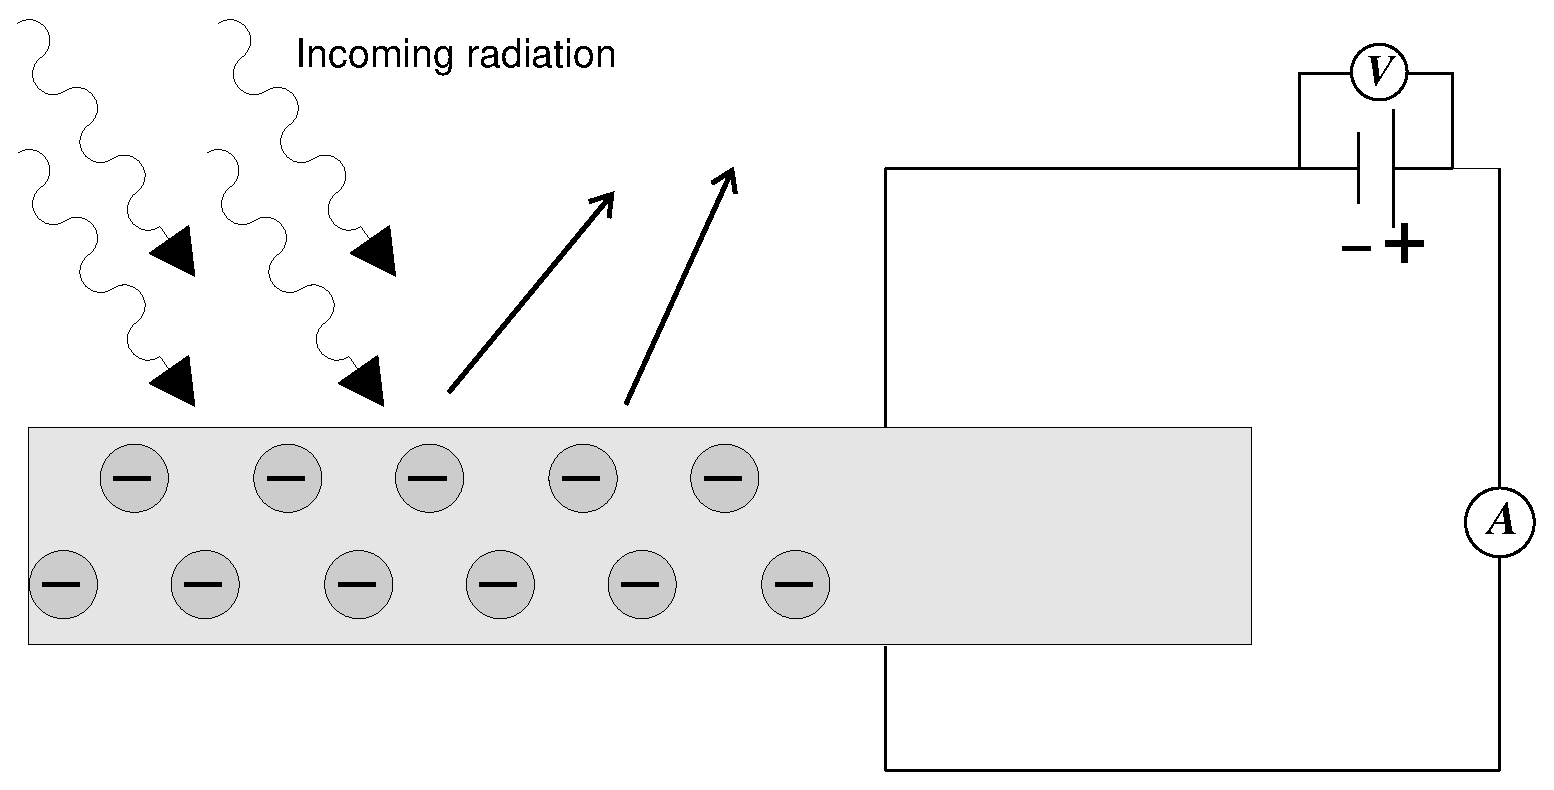
\includegraphics[width=0.4\textwidth]{../../epsimages/electFromSurface.eps}
%\caption{Diagram of a circuit to measure the photoelectric effect. If the photons on the left eject electrons from the metal foil, the metal %foil will lose some negative charge carriers. New negative charges will flow toward the metal foil to replace the lost electrons, and a current %will be measured by the ammeter in the circuit.}
%\label{elec_cir}
%\end{center}
%\end{figure}

We have learnt that a metal contains electrons that are free to move between the valence and conduction bands. When a photon strikes the surface of a metal, it gives \textit{all} its energy to one electron in the metal. 
\begin{itemize}
\item If the photon energy is \textit{equal} to the energy between two energy levels then the electron is excited to the higher energy level.
\item If the photon energy is \textit{greater} than or \textit{equal to} the work function (energy needed to escape from the metal), then the electron is emitted from the surface of the metal (the photoelectric effect). 
\end{itemize}

The work function is different for different elements. The smaller the work function, the easier it is for electrons to be emitted from the metal. Metals with low work functions make good conductors. This is because the electrons are attached less strongly to their surroundings and can move more easily through these materials. This reduces the resistance of the material to the flow of current i.e.\@ it conducts well. Table~\ref{tab:work_fun} shows the work functions for a range of elements.

\begin{table}[!h]
\begin{center}
\begin{tabular}{lc}
\hline
Element ~~~ & ~~~~ Work Function ($\mathrm{J}$) \\
\hline
Aluminium & ~~~ $6,9\times 10^{-19} $ \\
Beryllium & ~~~ $8,0 \times 10^{-19} $ \\
Calcium & ~~~ $4,6 \times 10^{-19} $ \\
Copper & ~~~ $7,5 \times 10^{-19}  $ \\
Gold & ~~~ $8,2 \times 10^{-19}  $ \\
Lead & ~~~ $6,9 \times 10^{-19}  $ \\
Silicon & ~~~ $1,8 \times 10^{-19}  $ \\
Silver & ~~~ $6,9 \times 10^{-19}  $ \\
Sodium & ~~~ $3,7 \times 10^{-19} $ \\
\hline
\end{tabular}
\caption{{ Work functions of selected elements determined from the photoelectric effect. (From the \it{Handbook of Chemistry and Physics.})}}
\label{tab:work_fun}
\end{center}
\end{table}


%Since, $E=hf$, we can calculate a minimum frequency $f_{min}$ of electromagnetic radiation that will cause an electron to be emitted from the %metal, where
%\nequ{f_{min}=\frac{E_{min}}{h}}. 
 

\begin{IFact}
{The \textbf{electron volt} (eV) is the kinetic energy gained by an electron  passing through a potential difference of one volt (1 $\mathrm{V}$). A \textbf{volt} is not a measure of energy, but the \textbf{electron volt} is a unit of energy. When you connect a $1.5 ~\mathrm{V}$ battery to a circuit, you can give $1.5~\mathrm{eV}$ of energy to every electron.}
\end{IFact}

%Suppose an electron in the metal needs $5~\mathrm{eV}$ of energy to escape the surface of the metal ($5~\mathrm{eV}$ is the binding energy of %the electron). And suppose a photon that interacts with the electron has just $2~\mathrm{eV}$ of energy in its energy packet. Then the electron %will not leave the surface of the metal. But suppose the photon has instead not $2~\mathrm{eV}$, but rather $8~\mathrm{eV}$ of energy. This %means that the electron will emerge from the metal, and it will also have some kinetic energy. The maximum kinetic energy that it can have is %$3~\mathrm{eV}$ when it leaves the surface.
% This does not mean the photon can give $5~\mathrm{eV}$ of energy to one electron and $3~\mathrm{eV}$ to another. A photon will give all of its %energy to just one electron.
%\begin{center}
%\psshadowbox{
%\begin{tabular}{rl}
%\multicolumn{2}{c}{$E_{k} = hf - \phi$} \\
%$E_{k}$&: maximum kinetic energy of the emitted electron $(\mathrm{J})$ or $(\mathrm{eV})$ \\
%$f$ &: frequency of the photon $(\mathrm{Hz})$ or $(\mathrm{s^{-1}})$ \\
%$h$ &: $6.57 \times 10^{-34} $ is Planck's constant $(\mathrm{J \cdot s}) $ \\
%or $h$ &: $4.14 \times 10^{-15} $ is also Planck's constant $(eV \cdot s) $ \\
%$\phi$ &: energy of the work function of the metal $(\mathrm{J})$ or $(\mathrm{eV})$\\
%\end{tabular}
%}
%\end{center}
%The minimum amount of energy needed for an electron to escape from a particular metal $E_{min}$, is called the work function of the metal. We %denote the work function of the metal by the Greek letter $\mathrm{\phi}$ ($\mathrm{phi}$). In our example, the work function is %$5~\mathrm{eV}$. The work function has a different value for each material: for example $4,70~\mathrm{eV}$ for copper and $2,28~\mathrm{eV}$ for %sodium. It is worth mentioning that the best conductors are those with the smallest work functions. This is why the photoelectric effect is most %easily measured by shining photons onto a metal.
%\begin{figure}
%\begin{center}
%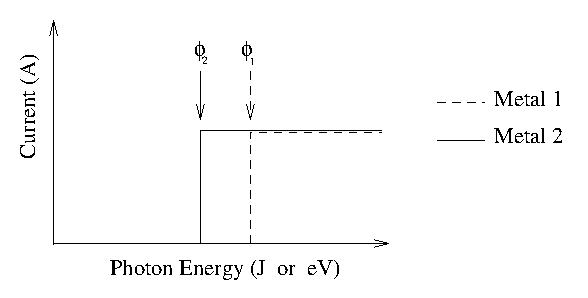
\includegraphics[width=0.6\textwidth]{../../epsimages/two_metals_2.eps}
%\caption{The current measured by the ammeter if the same light fall onto two different metals. These two metal have different work functions. %The metal with the lower work function $(\phi_{2})$ will measure a current with the ammeter at lower photon energies. This is because the %electrons need less energy to escape the surface.}
%\label{int_light_same}
%\end{center}
%\end{figure}
%\begin{figure}
%\begin{center}
%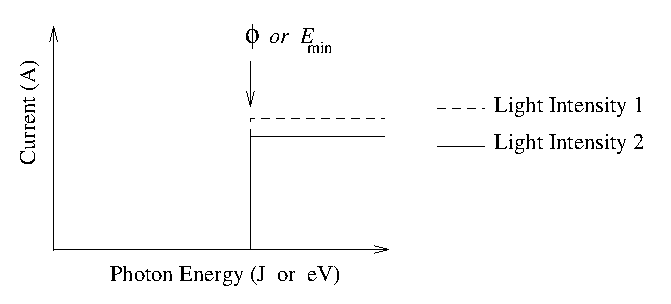
\includegraphics[width=0.6\textwidth]{../../epsimages/int_of_two_lights_2.eps}
%\caption{The current measured by the ammeter, if light of two different
%intensities falls onto the same type of metal. The greater the intensities of the light (or the greater the number of photons), the more %electrons are emitted from the metal. The emitted electrons will have the same energy for either of the two intensities. This is because the %energy of the emitted electrons depend on the energy of the photons, and not on the number of photons. }
%\label{int_light_diff}
%\end{center}
%\end{figure}

%The maximum kinetic energy acquired by the electron is equal
%to the energy of the photon minus the work function.
%The electrons emerge from the metal with a range of velocities from zero (when the photons have an energy equal to the work function) up to a
%maximum velocity $ v_{max}.$
%\begin{center}
%\psshadowbox{
%\begin{tabular}{rl}
%\multicolumn{2}{c}{ $E_{k} = hf - \phi = \frac{1}{2} m v_{max}^{2}$ } \\
%$E_{k}$ &: maximum kinetic energy of the emitted electron ($\mathrm{eV}$)\\
%$m$ &: the mass of the electron ($\mathrm{eV\cdot c^{-2}}$)\\
%$v_{max}$ &: the velocity of the emitted electron ($\mathrm{m\cdot s^{-1}}$) \\
%\end{tabular}
%}
%\end{center}

%The kinetic energy of the electron $E_k$ is directly proportional to the frequency of the radiation, and is independent of the intensity of the %light. For incoming radiation of a given frequency, the number of electrons emitted per unit time is proportional to the intensity of the %radiation. This can be shown in Fig~\ref{int_light_diff}.  The greater the intensity of the light shining on the metal, the greater the number %of electrons emitted, and hence the greater the current that is measured.
% Another important feature of the photoelectric effect, is that the electron emission takes place from the instant the light shines on the %surface, i.e.\@ there is no detectable time delay.  This finding was unexpected. Classical theory predicted that the electrons would pick up %energy over a period of time, like the heating effect, and then be emitted. The photoelectric effect, since the electrons were emitted %instantaneously, could therefore not be explained by classical theories.  It could only be explained by assuming that each photon behaved like a %particle of light, giving all its energy instantaneously to one electron.  
%We have shown that light can act as a wave with a characteristic wavelength and frequency. This was also studied in the previous chapters on %waves \ref{chap:pw} and optics \ref{chap:optics}.  In this chapter we have studied that light can also acts as a bunch of discrete particles %each with a bundle of energy related to the frequency.  
%\begin{figure}
%\begin{center}
%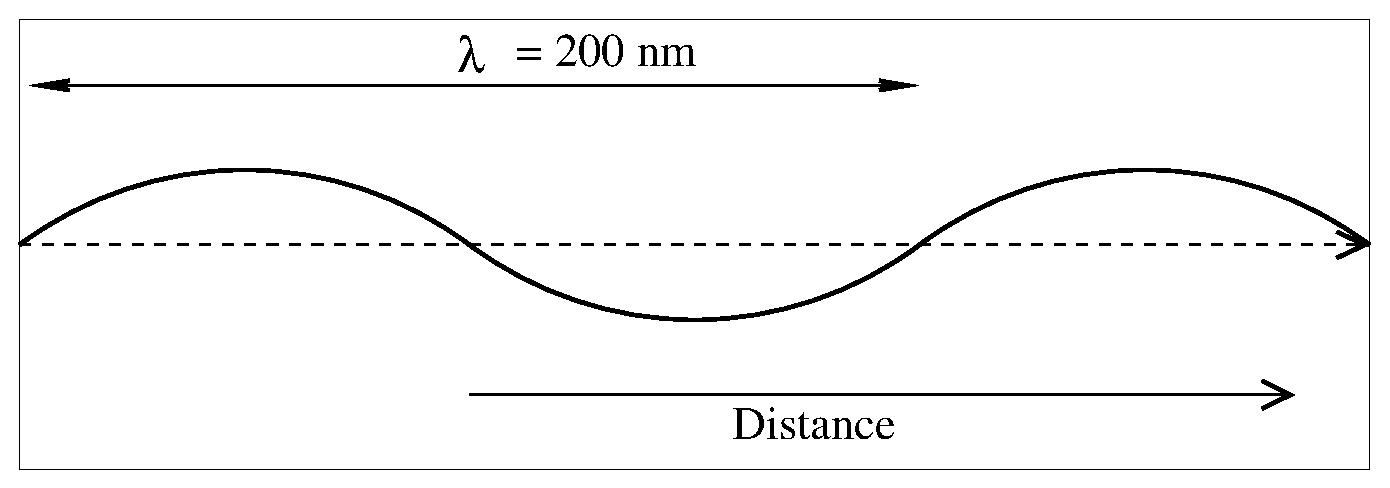
\includegraphics[width=0.4\textwidth]{../../epsimages/wave_wavelength.eps}
%\caption{Ultraviolet radiation has a wavelength of 200~nm}
%\label{int_light}
%\end{center}
%\end{figure}

%\begin{IFact}
%{It is worth mentioning that the best conductors are those with the smallest work functions. There is a very logical explanation to this. A %smaller value of the work function means that the electron is attached less strongly to its surroundings and thus it is easier for the electron %to move around inside the metal. This reduces its resistance to the flow of current.}
%\end{IFact}

\begin{wex}{The photoelectric effect - I}
{Ultraviolet radiation with a wavelength of 250~nm is incident on a silver foil (work function $\phi$ = $6,9 \times 10^{-19}$). What is the maximum kinetic energy of the emitted electrons?}
{\westep{Determine what is required and how to approach the problem}
We need to determine the maximum kinetic energy of an electron ejected from a silver foil by ultraviolet radiation. 

The photoelectric effect tells us that:
\begin{eqnarray*}
E_{k} & = & E_{photon} - \phi \\
E_k & = & h\frac{c}{\lambda}-\phi
\end{eqnarray*}

We also have: \\
Work function of silver: $\phi =6,9 \times 10^{-19}$ J  \\
UV radiation wavelength = 250~nm = $250 \times 10^{-9}$ m \\
Planck's constant: $h = 6,63 \times 10^{-34}~~\rm{m^{2}}\rm{kg}\rm{s^{-1}}$ \\
speed of light: $c = 3 \times 10^{8}~\rm{m}\rm{s^{-1}}$ \\

\westep{Solve the problem}
\begin{eqnarray*}
E_{k} & = & \frac{hc}{\lambda} - \phi \\
& = & [6,63 \times 10^{-34} \times \frac{3\times10^{8}}{250\times10^{-9}}] - 6,9 \times 10^{-19} \\
& = & 1,06 \times 10^{-19}~\rm{J}
\end{eqnarray*}

The maximum kinetic energy of the emitted electron will be $1,06 \times 10^{-19}~\rm{J}$.}
\end{wex}



\begin{wex}{The photoelectric effect - II}
{If we were to shine the same ultraviolet radiation ($f = 1,2 \times 10^{15}~\rm{Hz}$), on a gold foil (work function $= 8,2 \times 10^{-19}~\mathrm{J}$), would any electrons be emitted from the surface of the gold foil?}
{
For the electrons to be emitted from the surface, the energy of each photon needs to be \textit{greater} than the work function of the material. 
\westep{Calculate the energy of the incident photons}
\begin{eqnarray*}
E_{photon}& = & hf \\
& = & 6,63 \times 10^{-34} \times 1,2 \times 10^{15} \\
& = & 7,96 \times 10^{-19}~\rm{J}\\
\end{eqnarray*}

Therefore each photon of ultraviolet light has an energy of $7,96 \times 10^{-19}~\rm{J}$.

\westep{Write down the work function for gold.}
\begin{eqnarray*}
\phi_{gold} & = & 8,2 \times 10^{-19}~\mathrm{J} \\
\end{eqnarray*}

\westep{Is the energy of the photons greater or smaller than the work function?}

\begin{eqnarray*}
7,96 \times 10^{-19}~\rm{J} & < & 8,2 \times 10^{-19}~\mathrm{J}  \\
E_{photons} & < & \phi_{gold} \\
\end{eqnarray*}

The energy of each photon is less than the work function of gold, therefore, the photons do not have enough energy to knock electrons out of the gold. No electrons would be emitted from the gold foil.}
\end{wex}


\Extension{Units of energy}{
When dealing with calculations at a small scale (like at the level of electrons) it is more convenient to use different units for energy rather than the joule (J). We define a unit called the electron-volt (eV) as the kinetic energy gained by an electron passing through a potential difference of one volt. 
\nequ{E = q \times V}
where $q$ is the charge of the electron and $V$ is the potential difference applied. The charge of 1 electron is $1,6 \times 10^{-19}$~C, so 1~eV is calculated to be:
\nequ{1\;\mathrm{eV}= (1,6  10^{-19}\;\mathrm{C} \times 1\;\mathrm{V}) =1,6 \times 10^{-19}\eJ}

\noindent You can see that  $1,6 \times 10^{-19}$ J is a very small amount of energy and so using electron-volts (eV) at this level is easier.

\noindent Hence, 1eV = $1.6 \times 10^-19$ J which means that 1 J = $6.241 \times 10^{18}$ eV
}

%\begin{IFact}
%{Max Karl Ernst Ludwig Planck (23 April 1858 -- 4 October 1947) was one of the most  important German physicists of the late nineteenth and %early twentieth century. He is considered to be one of the founders of quantum theory. He received a Nobel prize for physics in 1918 for %recognition of the services he rendered to the advancement of Physics by his discovery of energy quanta. Planck's constant ($h$) is named after %Max Planck.}
%\end{IFact}

%\begin{IFact}
%{Albert Einstein (14 March 1879 -- 18 April 1955) was a theoretical physicist, widely regarded as the most important scientist of the twentieth %century. He made major contributions to the special and general theories of relativity and made significant contributions to quantum mechanics, %statistical mechanics, and cosmology. He was awarded the 1921 Nobel Prize for Physics for his explanation of the photoelectric effect in 1905 %and for his services to Theoretical Physics.}
%\end{IFact}

%\subsection{Relation to De Broglie's hypothesis}
%The dual-nature of light has an intricate relation with De Broglie's hypothesis. Recall that the wavelength of matter waves is given by:
%$\lambda= h/p$
%where	$\lambda$ is the wavelength of the matter wavelength, $h$ is Planck's constant and $p$ is the momentum of the body.
%De Broglie's equation gives us the wavelength of any object that has velocity (and thus momentum). Conversely, it also leads us to the idea of %electromagnetic waves possessing momentum (by just writing the equation as $p=\frac{h}{\lambda}$, where $\lambda$ is the wavelength of the %wave). This led to the idea of waves having mass, which is totally misleading. Photons do possess momentum according to several experiments, but %the existence of mass has never been established. We will assume that photons possess momentum (and not worry about whether they have mass or %not!).
 
%\begin{IFact}
%{The fact that waves have momentum has been put to some very innovative practical use. You might have heard of solar sails; several space %agencies are thinking of using them in the propulsion of space vehicles. This would use the change in momentum of light photons from the Sun %which are deflected back after striking the reflective surface of the sail. The force due to this change in momentum could be used to provide %thrust for the spacecraft.}
%\end{IFact}


\subsection{Real-life applications}
\subsubsection{Solar Cells}
The photo-electric effect may seem like a very easy way to produce electricity from the sun.
This is why people choose to make solar panels out of materials like silicon, to generate electricity. 
In real-life however, the amount of electricity generated is less than expected. This is because not every photon knocks out an electron. Other  processes such as reflection or scattering also happen. This means that only a fraction $\approx 10\%$ (depends on the material) of the photons produce photoelectrons. This drop in efficiency results in a lower current. Much work is being done in industry to improve this efficiency so that the panels can generate as high a current as possible, and create as much electricity as possible from the sun. But even these smaller electrical currents are useful in applications like solar-powered calculators.
 
\Exercise{The photoelectric effect}{
\begin{enumerate}
\item{Describe the photoelectric effect.}
\item{List two reasons why the observation of the photoelectric effect was significant.}
\item{Refer to Table~\ref{tab:work_fun}: If I shine ultraviolet light with a wavelength of 288~nm onto some aluminium foil, what would be the kinetic energy of the emitted electrons? }
\item{I shine a light of an unknown wavelength onto some silver foil. The light has only enough energy to eject electrons from the silver foil but not enough to give them kinetic energy. (Refer to Table~\ref{tab:work_fun} when answering the questions below:)
  \begin{enumerate}
  \item If I shine the same light onto some copper foil, would electrons be ejected? 
  \item If I shine the same light onto some silicon, would electrons be ejected?
  \item If I increase the intensity of the light shining on the silver foil, what happens?
  \item If I increase the frequency of the light shining on the silver foil, what happens?
  \end{enumerate} }
\end{enumerate}

% Automatically inserted shortcodes - number to insert 4
\par \practiceinfo
\par \begin{tabular}[h]{cccccc}
% Question 1
(1.)	01mq	&
% Question 2
(2.)	01mr	&
% Question 3
(3.)	01ms	&
% Question 4
(4.)	01mt	&
\end{tabular}
% Automatically inserted shortcodes - number inserted 4
}




\section{Emission and absorption spectra}

\subsection{Emission Spectra}

You have learnt previously about the structure of an atom.  The electrons surrounding the atomic nucleus are arranged in a series of levels of increasing energy.  Each element has its own distinct set of energy levels.  This arrangement of energy levels serves as the atom's unique fingerprint.
 
In the early 1900s, scientists found that a liquid or solid heated to high temperatures would give off a broad range of colours of light. However, a gas heated to similar temperatures would emit light only at certain specific colours (wavelengths).  The reason for this observation was not understood at the time.\\  
 
Scientists studied this effect using a discharge tube.  

\begin{figure}[H]
\begin{center}
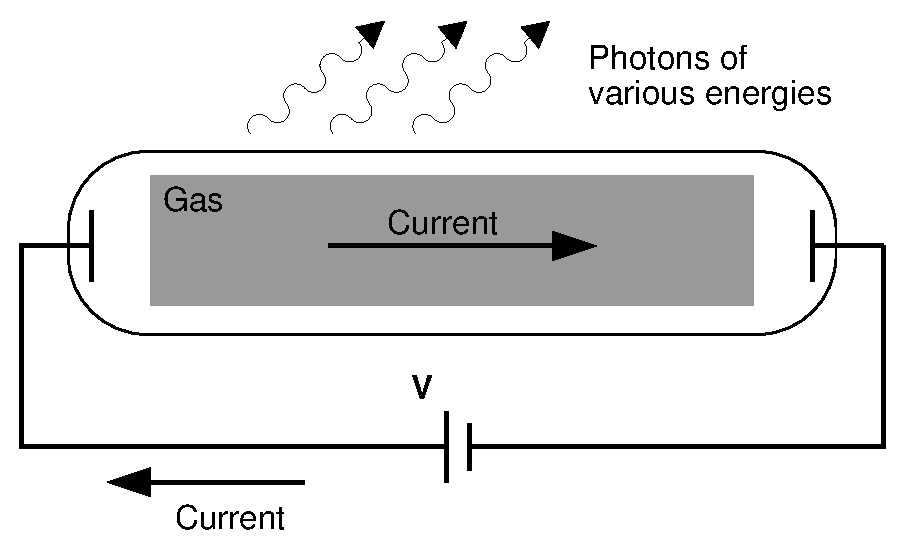
\includegraphics[width=4.in]{../../epsimages/discharge_tube.eps}
\end{center}
\caption{Diagram of a discharge tube.  The tube is filled with a gas.  When a high enough voltage is applied across the tube, the gas ionises and acts like a conductor, allowing a current to flow through the circuit.  The current excites the atoms of the ionised gas.  When the atoms fall back to their ground state, they emit photons to carry off the excess energy.}
\label{dischargetube}
\end{figure}


A discharge tube (Figure~\ref{dischargetube}) is a glass gas-filled tube with a metal plate at both ends. If a large enough voltage difference is applied between the two metal plates, the gas atoms inside the tube will absorb enough energy to make some of their electrons come off i.e.\@ the gas atoms are ionised. These electrons start moving through the gas and create a current, which raises some electrons in other atoms to higher energy levels. Then as the electrons in the atoms fall back down, they emit electromagnetic radiation (light). The amount of light emitted at different wavelengths, called the \textbf{emission spectrum}, is shown for a discharge tube filled with hydrogen gas in figure~\ref{hydrogenspectrum} below. Only certain wavelengths (i.e.\@ colours) of light are seen as shown by the thick black lines in the picture.

\begin{figure}[H]
\begin{center}
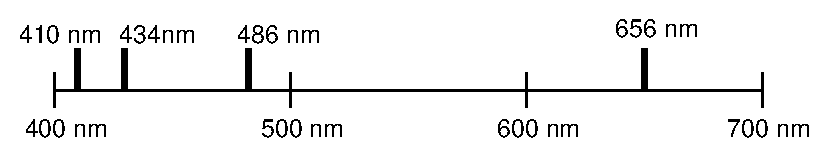
\includegraphics[width=4.5in]{../../epsimages/hydrogen_emission_spectrum.eps}
\end{center}
\caption{Diagram of the emission spectrum of hydrogen in the visible spectrum.  Four lines are visible, and are labelled with their wavelengths.  The three lines in the 400--500 nm range are in the blue part of the spectrum, while the higher line (656 nm) is in the red/orange part.}
\label{hydrogenspectrum}
\end{figure}

Eventually, scientists realised that these lines come from photons of a specific energy, emitted by electrons making transitions between specific energy levels of the atom.  Figure~\ref{ig:Henergy} shows an example of this happening.  When an electron in an atom falls from a higher energy level to a lower energy level, it emits a photon to carry off the extra energy.  This photon's energy is equal to the energy difference between the two energy levels.  As we previously discussed, the frequency of a photon is related to its energy through the equation $E=hf$.  Since a specific photon frequency (or wavelength) gives us a specific colour, we can see how each coloured line is associated with a specific transition. 
 
%\begin{figure}[H]
%\begin{center}
%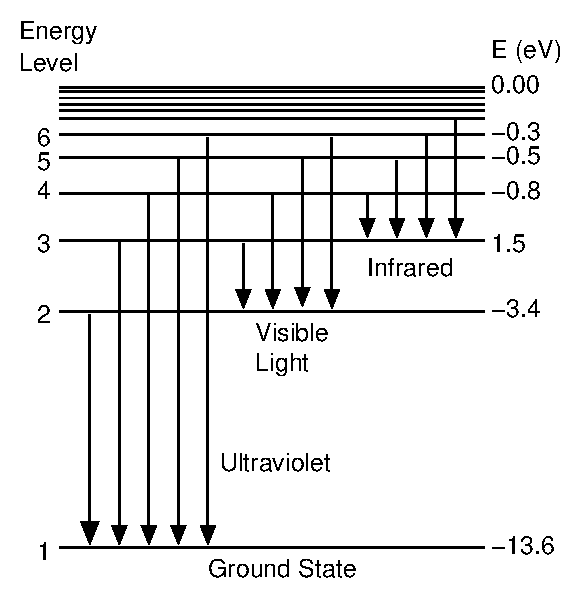
\includegraphics[width=3.5in]{../../epsimages/hydrogen_transitions.eps}
%\caption{In this diagram, various energy levels of the hydrogen atom are shown, with the associated transitions between these levels.  Each %transition gives off a photon with a distinct energy.  Each set of transitions lies in a different area of the electromagnetic spectrum.  For %example, the transitions to the ground state give off ultraviolet radiation; the transitions down to the first excited state (second energy %level) give off visible light; the transitions to the second excited state give off ultraviolet radiation.}
%\label{hydrogen-emission-diagram}
%\end{figure}

\begin{figure}[H]
\begin{center}
\scalebox{1} % Change this value to rescale the drawing.
{
\begin{pspicture}(0,-3.1)(10.66,3.1)
\psline[linewidth=0.04cm](0.7,-2.9)(7.48,-2.9)
\psline[linewidth=0.04cm](0.7,-0.08)(7.48,-0.08)
\psline[linewidth=0.04cm](0.7,0.54)(7.48,0.54)
\psline[linewidth=0.04cm](0.68,1.06)(7.46,1.06)
\psline[linewidth=0.04cm](0.66,1.54)(7.44,1.54)
\psline[linewidth=0.04cm](0.68,1.84)(7.46,1.84)
\psline[linewidth=0.04cm](0.68,2.04)(7.46,2.04)
\psline[linewidth=0.04cm](0.68,2.16)(7.46,2.16)
\psline[linewidth=0.04cm](0.68,2.26)(7.46,2.26)
\psline[linewidth=0.04cm](0.68,2.34)(7.46,2.34)
\rput(0.52,2.925){Energy}
\rput(0.49,2.605){Level}
\rput(0.51,-2.855){1}
\rput(0.51,-0.055){2}
\rput(0.52,0.545){3}
\rput(0.53,1.065){4}
\rput(0.52,1.545){5}
\rput(0.53,1.865){6}
\rput(0.51,2.345){\small $\infty$}
\rput(7.76,-2.915){\small 0 J}
\rput(8.78,-0.075){\small $16,3 \times 10^{-19}$ J}
\rput(8.8,0.565){\small $19,4 \times 10^{-19}$ J}
\rput(8.82,1.065){\small $20,5 \times 10^{-19}$ J}
\rput(8.82,1.545){\small $21,0 \times 10^{-19}$ J}
\rput(8.82,2.365){\small $21,8 \times 10^{-19}$ J}
\rput(8.84,1.825){\small $21,3 \times 10^{-19}$ J}
\psline[linewidth=0.03cm,arrowsize=0.05291667cm 2.0,arrowlength=1.4,arrowinset=0.4]{->}(1.08,-0.08)(1.1,-2.94)
\psline[linewidth=0.03cm,arrowsize=0.05291667cm 2.0,arrowlength=1.4,arrowinset=0.4]{->}(1.38,0.56)(1.4,-2.94)
\psline[linewidth=0.03cm,arrowsize=0.05291667cm 2.0,arrowlength=1.4,arrowinset=0.4]{->}(1.7,1.02)(1.7,-2.92)
\psline[linewidth=0.03cm,arrowsize=0.05291667cm 2.0,arrowlength=1.4,arrowinset=0.4]{->}(1.98,1.54)(2.0,-2.92)
\psline[linewidth=0.03cm,arrowsize=0.05291667cm 2.0,arrowlength=1.4,arrowinset=0.4]{->}(2.3,1.8)(2.32,-2.92)
\psline[linewidth=0.03cm,arrowsize=0.05291667cm 2.0,arrowlength=1.4,arrowinset=0.4]{->}(3.46,0.56)(3.48,-0.12)
\psline[linewidth=0.03cm,arrowsize=0.05291667cm 2.0,arrowlength=1.4,arrowinset=0.4]{->}(3.74,1.06)(3.74,-0.1)
\psline[linewidth=0.03cm,arrowsize=0.05291667cm 2.0,arrowlength=1.4,arrowinset=0.4]{->}(4.06,1.52)(4.06,-0.1)
\psline[linewidth=0.03cm,arrowsize=0.05291667cm 2.0,arrowlength=1.4,arrowinset=0.4]{->}(4.32,1.82)(4.36,-0.1)
\psline[linewidth=0.03cm,arrowsize=0.05291667cm 2.0,arrowlength=1.4,arrowinset=0.4]{->}(5.32,1.08)(5.34,0.46)
\psline[linewidth=0.03cm,arrowsize=0.05291667cm 2.0,arrowlength=1.4,arrowinset=0.4]{->}(5.58,1.5)(5.58,0.5)
\psline[linewidth=0.03cm,arrowsize=0.05291667cm 2.0,arrowlength=1.4,arrowinset=0.4]{->}(5.9,1.8)(5.9,0.5)
\psline[linewidth=0.03cm,arrowsize=0.05291667cm 2.0,arrowlength=1.4,arrowinset=0.4]{->}(6.22,2.0)(6.22,0.52)
\rput(3.14,-2.095){ultraviolet}
\rput(3.92,-0.395){visible light}
\rput(5.75,0.245){infrared}
\rput(9.01,-2.875){\small ground state}
\rput(8.06,2.905){Energy}
\end{pspicture} 
}
\end{center}
\caption{In this diagram are shown some of the electron energy levels for the hydrogen atom. The arrows show the electron transitions from higher energy levels to lower energy levels. The energies of the emitted photons are the same as the energy difference between two energy levels. You can think of absorption as the opposite process. The arrows would point upwards and the electrons would jump up to higher levels when they absorb a photon of the right energy.  }
\label{fig:Henergy}
\end{figure}


Visible light is not the only kind of electromagnetic radiation emitted. More energetic or less energetic transitions can produce ultraviolet or infrared radiation. However, because each atom has its own distinct set of energy levels (its fingerprint!), each atom has its own distinct emission spectrum.



 
\subsection{Absorption spectra}

As you know, atoms do not only emit photons; they also absorb photons. If a photon hits an atom and the energy of the photon is the same as the gap between two electron energy levels in the atom, then the electron can absorb the photon and jump up to the higher energy level. If the atom has no energy level differences that equal the incoming photon's energy, it cannot absorb the photon, and can only scatter it.
 
Using this effect, if we have a source of photons of various energies we can obtain the \textbf{absorption spectra} for different materials. To get an absorption spectrum, just shine white light on a sample of the material that you are interested in. White light is made up of all the different wavelengths of visible light put together. In the absorption spectrum, the energy levels corresponding to the absorbed photons show up as black lines because the photons of these wavelengths have been absorbed and don't show up. Because of this, the absorption spectrum is the exact \textit{inverse} of the emission spectrum. Look at the two figures below. In figure~\ref{fig:emissionSpec} you can see the emission lines of hydrogen. Figure~\ref{fig:absorptionSpec} shows the absorption spectrum. It is the exact opposite of the emission spectrum! Both emission and absorption techniques can be used to get the same information about the energy levels of an atom.

\begin{figure}[H]
\begin{pspicture}(\linewidth,1.1)
\psspectrum[element=H,lwidth=0.1](\linewidth,1)
\end{pspicture}
\caption{\textit{Emission} spectrum of Hydrogen.}\label{fig:emissionSpec}
\end{figure}

\begin{figure}[H]
\begin{pspicture}(\linewidth,1.1)
\psspectrum[absorption,element=H,lwidth=0.1](\linewidth,1)
\end{pspicture}
\caption{\textit{Absorption} spectrum of Hydrogen.}\label{fig:absorptionSpec}
\end{figure}



\begin{wex}{Absorption}
{I have an unknown gas in a glass container. I shine a bright white light through one side of the container and measure the spectrum of transmitted light. I notice that there is a black line (\textit{absorption} line) in the middle of the visible red band at 642 nm. I have a hunch that the gas might be hydrogen. If I am correct, between which 2 energy levels does this transition occur? (Hint: look at figure~\ref{fig:Henergy} and the transitions which are in the visible part of the spectrum.)
}
{\westep{What is given and what needs to be done?}
We have an absorption line at 642 nm. This means that the substance in the glass container absorbed photons with a wavelength of 642 nm. 
We need to calculate which 2 energy levels of hydrogen this transition would correspond to. Therefore we need to know what energy the absorbed photons had.

\westep{Calculate the energy of the absorbed photons}
\begin{eqnarray*}
E &=& \frac{hc}{\lambda} \\
  &=& \frac{(6,63 \times 10^{-34}) \times (3\times10^{8})}{642\times10^{-9}}\\
  &=& 3,1 \times 10^{-19}~~\rm{J}
\end{eqnarray*}
The absorbed photons had energy of $3,1 \times 10^{-19}$

\westep{Find the energy of the transitions resulting in radiation at visible wavelengths}
Figure~\ref{fig:Henergy} shows various energy level transitions. The transitions related to visible wavelengths are marked as the transitions beginning or ending on Energy Level 2. 
Let's find the energy of those transitions and compare with the energy of the absorbed photons we've just calculated.

Energy of transition (absorption) from Energy Level 2 to Energy Level 3:
\begin{eqnarray*}
E_{2,3} &=& E_{2} - E_{3}\\
&=& 16,3 \times 10^{-19}~~\rm{J} - 19,4 \times 10^{-19}~~\rm{J}\\
&=& -3,1 \times 10^{-19}~~\rm{J}
\end{eqnarray*}
Therefore the energy of the photon that an electron must absorb to jump from Energy Level 2 to Energy Level 3 is $3,1 \times 10^{-19}~~\rm{J}$.
(NOTE: The minus sign means that \textit{absorption} is occurring.)

This is the same energy as the photons which were absorbed by the gas in the container! Therefore, since the transitions of all elements are unique, we can say that the gas in the container is hydrogen. The transition is absorption of a photon between Energy Level 2 and Energy Level 3.

}
\end{wex}



\subsection{Colours and energies of electromagnetic radiation}
We saw in the explanation for why the sky is blue that different \textit{wavelengths} or \textit{frequencies} of light correspond to different \textit{colours} of light. The table below gives the wavelengths and colours of light in the visible spectrum:

\begin{table}[H]
\begin{center}
\begin{tabular}{ | l | c |}
\hline
\textbf{Colour} & \textbf{Wavelength range (nm)} \\ \hline \hline
 violet   & 390 - 455  \\ \hline
 blue   &   455 -  492       \\ \hline
 green  &   492 - 577        \\ \hline
 yellow  &  577 - 597       \\ \hline
 orange  &  597 - 622        \\ \hline
 red  &    622 - 780         \\ \hline
\hline
\end{tabular}
\end{center}
\caption{Colours and wavelengths of light in the visible spectrum.}
\label{t:Optic:Colours}
\end{table}

We also know that the energy of a photon of light can be found from:
\begin{eqnarray*}
E & = &hf = \frac{hc}{\lambda} 
\end{eqnarray*}
Therefore if we know the frequency or wavelength of light, we can calculate the photon's energy and vice versa. 

\Activity{Investigation}{Frequency, wavelength and energy relation}
{
\noindent Refer to table~\ref{t:Optic:Colours}: Copy the table into your workbook and add two additional columns.
\begin{enumerate}
\item In the first new column write down the lower and upper frequencies for each colour of light. 
\item In the second column write down the energy range (in Joules) for each colour of light.
\end{enumerate}
\textbf{Questions}\\
\begin{enumerate}
\item Which colour of visible light has the highest energy photons?
\item Which colour of visible light has the lowest energy photons?
\end{enumerate} 
}
Discharge lamps (sometimes incorrectly called neon lights) use the spectra of various elements to produce light of many colours.

% PhET simulation on discharge lamps: SIYAVULA-SIMULATION:http://cnx.org/content/m39553/latest/#id6358

\simulation{Discharge lamps}{VPqea}

\begin{wex}{Colours of light}
{A photon of wavelength 500 nm is emitted by a traffic light. 
\begin{enumerate}
\item What is the energy of the photon?
\item What is the frequency of the photon?
\item Use table~\ref{t:Optic:Colours} to determine the colour of the light.
\end{enumerate}
}
{
\westep{What information is given and what do we need to find?}
We are given $\lambda = 500 \times 10^{-9}~~\rm{m}$ and we need to find the photon's \textit{energy}, \textit{frequency} and \textit{colour}.

\westep{Use the equation $E = \frac{hc}{\lambda}$ to find the photon's energy}
\begin{eqnarray*}
E & = & \frac{hc}{\lambda} \\
& = & \frac{(6,63 \times 10^{-34}) \times (3 \times 10^{8})}{ 500 \times 10^{-9}} \\
& = & 3,98 \times 10^{-19}~~\rm{J}
\end{eqnarray*}
The energy of the photon is $3,98\times10^{-19}$ J.

\westep{We know the energy of the photon, now we can use $E=hf$ to solve for the frequency}
\begin{eqnarray*}
E & = & hf \\
f & = & \frac{E}{h} \\
  & = & \frac{3.98 \times 10^{-19}}{6,63 \times 10^{-34}}\\
  & = & 6 \times 10^{14}~~\rm{Hz}
\end{eqnarray*}
The frequency of the photon is $6 \times 10^{14}~~\rm{Hz}$.

\westep{Use the table to find the colour of light}
The wavelength given in the question is 500 nm. We can see in the table that green light has wavelengths between 492 - 577 nm. Therefore 500 nm is in this range so the colour of the light is \textbf{green}.

}
\end{wex}

\begin{wex}{Colours and energies of light}
{I have some sources which emit light of the following wavelengths:
\begin{enumerate} 
\item 400 nm, 
\item 580 nm, 
\item 650 nm,
\item 300 nm.
\end{enumerate}
What are the colours of light emitted by the sources (see table~\ref{t:Optic:Colours})? Which source emits photons with the highest energy and which with the lowest energy?
}
{
\westep{What information is given, and what do we need to do?}
Four wavelengths of light are given and we need to find their \textit{colours}. 

We also need to find which colour photon has the highest energy and which one has the lowest energy.

\westep{To find the colours of light, we can compare the wavelengths to those given in table~\ref{t:Optic:Colours}}
\begin{enumerate}
 \item 400 nm falls into the range for \textit{violet} light (390 - 455 nm).
 \item 580 nm falls into the range for \textit{yellow} light (577 - 597 nm).
 \item 650 nm falls into the range for \textit{red} light (622 - 780 nm).
 \item 300 nm is not shown in the table. However, this wavelength is just a little shorter than the shortest wavelength in the violet range. Therefore 300 nm is \textit{ultraviolet}.
\end{enumerate}

\westep{To find the colour of the light whose photons have the highest and lowest energies respectively, we need to calculate the energies of all the photons}

We know $E = \frac{hc}{\lambda}$

\begin{minipage}{0.3\textwidth}
For 400 nm:
\begin{eqnarray*}
E & = & \frac{hc}{\lambda} \\
  & = & \frac{(6,63 \times 10^{-34}) \times (3 \times 10^{8}) }{400 \times 10^{-9}} \\
  & = &  4,97 \times 10^{-19}~~\rm{J}
\end{eqnarray*}
\end{minipage}

\begin{minipage}{0.3\textwidth}
For 580 nm:
\begin{eqnarray*}
E & = & \frac{hc}{\lambda} \\
  & = & \frac{(6,63 \times 10^{-34}) \times (3 \times 10^{8}) }{580 \times 10^{-9}} \\
  & = &  3,43 \times 10^{-19}~~\rm{J}
\end{eqnarray*}
\end{minipage}

\begin{minipage}{0.3\textwidth}
For 650 nm:
\begin{eqnarray*}
E & = & \frac{hc}{\lambda} \\
  & = & \frac{(6,63 \times 10^{-34}) \times (3 \times 10^{8}) }{650 \times 10^{-9}} \\
  & = &  3,06 \times 10^{-19}~~\rm{J}
\end{eqnarray*}
\end{minipage}

\begin{minipage}{0.3\textwidth}
For 300 nm:
\begin{eqnarray*}
E & = & \frac{hc}{\lambda} \\
  & = & \frac{(6,63 \times 10^{-34}) \times (3 \times 10^{8}) }{300 \times 10^{-9}} \\
  & = &  6,63 \times 10^{-19}~~\rm{J}
\end{eqnarray*}
\end{minipage}

Therefore, the photons with the highest energy are the \textbf{ultraviolet} photons. \\
The photons with the lowest energy are from light which is \textbf{red}.

}
\end{wex}



\subsection{Applications of emission and absorption spectra}
The study of spectra from stars and galaxies in astronomy is called \textit{spectroscopy}. Spectroscopy is a tool widely used in astronomy to learn different things about astronomical objects.

\subsubsection{Identifying elements in astronomical objects using their spectra}
Measuring the spectrum of light from a star can tell astronomers what the star is made of! Since each element emits or absorbs light only at particular wavelengths, astronomers can identify what elements are in the stars from the lines in their spectra. From studying the spectra of many stars we know that there are many different types of stars which contain different elements and in different amounts.

%\textit{Nebulae} are enormous clouds of gas and dust in our galaxy which are thought to be the birth places of stars. Astronomers have been able %to deduce that most of the gas in these clouds is hydrogen gas (ionised) by identifying the emission lines in the spectra of these objects.

\subsubsection{Determining velocities of galaxies using spectroscopy}
You have already learnt in Chapter~\ref{p:wsl:de12} about the Doppler effect and how the frequency (and wavelength) of sound waves changes depending on whether the object emitting the sound is moving \textit{towards} or \textit{away} from you. The same thing happens to electromagnetic radiation (light). If the object emitting the light is moving \textit{towards} us, then the wavelength of the light appears shorter (called \textbf{blue-shifted}). If the object is moving \textit{away} from us, then the wavelength of its light appears stretched out (called \textbf{red-shifted}). 

The Doppler effect affects the spectra of objects in space depending on their motion relative to us on the earth. For example, the light from a distant galaxy, which is moving away from us at some velocity, will appear red-shifted. This means that the emission and absorption lines in the galaxy's spectrum will be shifted to a longer wavelength (lower frequency). Knowing where each line in the spectrum would normally be if the galaxy was not moving, and comparing to their red-shifted positions, allows astronomers to precisely measure the velocity of the galaxy relative to the earth!



\subsubsection{Global warming and greenhouse gases}
The sun emits radiation (light) over a range of wavelengths which are mainly in the visible part of the spectrum. Radiation at these wavelengths passes through the gases of the atmosphere to warm the land and the oceans below. The warm earth then radiates this heat at longer infrared wavelengths. Carbon-dioxide (one of the main greenhouse gases) in the atmosphere has energy levels which correspond to the infrared wavelengths which allow it to absorb the infrared radiation. It then also emits at infrared wavelengths in all directions. This effect stops a large amount of the infrared radiation getting out of the atmosphere, which causes the atmosphere and the earth to heat up. More radiation is coming in than is getting back out.    

\begin{center}
\scalebox{1} % Change this value to rescale the drawing.
{
\begin{pspicture}(0,-2.59)(15.975868,2.57)
\psbezier[linewidth=0.04](3.4958684,2.53)(3.5758684,1.85)(5.2958684,1.75)(5.4158683,2.55)
\psline[linewidth=0.04cm](3.5158684,2.23)(3.1158683,1.89)
\psline[linewidth=0.04cm](3.8358684,1.99)(3.5558684,1.59)
\psline[linewidth=0.04cm](4.1958685,1.93)(4.1358685,1.47)
\psline[linewidth=0.04cm](4.5758686,1.93)(4.6358685,1.43)
\psline[linewidth=0.04cm](4.9558682,1.99)(5.1358685,1.57)
\psline[linewidth=0.04cm](5.3358684,2.21)(5.7158685,1.79)
\psbezier[linewidth=0.04,arrowsize=0.05291667cm 2.0,arrowlength=1.4,arrowinset=0.4]{->}(5.3158684,-1.8245102)(5.4166245,-1.808687)(5.439445,-1.2557855)(5.6350846,-1.3248497)(5.830724,-1.393914)(5.9961104,-1.0932733)(5.831161,-0.9905677)(5.666211,-0.8878622)(5.878371,-0.53134257)(6.0578475,-0.6263778)(6.2373247,-0.7214131)(6.42343,-0.38185132)(6.2439528,-0.28681606)(6.064476,-0.19178078)(6.281192,0.17768885)(6.4606686,0.082653575)(6.640146,-0.012381695)(6.358866,-0.0017902247)(6.759594,0.57)
\psbezier[linewidth=0.03,arrowsize=0.05291667cm 2.0,arrowlength=1.4,arrowinset=0.4]{->}(4.266691,1.9676449)(4.4793305,1.9886502)(4.4655175,1.7896867)(4.310693,1.7585212)(4.1558685,1.7273557)(4.168905,1.5119989)(4.3296576,1.5552567)(4.4904103,1.5985147)(4.5284834,1.3772986)(4.3832135,1.3371572)(4.237943,1.2970159)(4.2414255,1.090635)(4.4099193,1.1354511)(4.578413,1.1802672)(4.579593,0.9407257)(4.455734,0.9157933)(4.331874,0.89086086)(4.3371696,0.6739458)(4.5015483,0.69613546)(4.665927,0.71832514)(4.6848917,0.5150607)(4.530067,0.4838952)(4.3752427,0.4527297)(4.40969,0.2525818)(4.5740685,0.2747715)(4.738447,0.2969612)(4.72826,0.07692955)(4.579364,0.05785641)(4.4304676,0.03878328)(4.48221,-0.16878216)(4.6311064,-0.14970903)(4.7800026,-0.13063589)(4.8203783,-0.3186914)(4.667367,-0.36039102)(4.514355,-0.4020906)(4.564285,-0.5991219)(4.709555,-0.55898064)(4.8548255,-0.5188393)(4.90064,-0.7384971)(4.7458153,-0.7696626)(4.590991,-0.8008281)(4.6368055,-1.0204859)(4.79163,-0.9893204)(4.9464545,-0.9581549)(4.967232,-1.1719534)(4.818336,-1.1910266)(4.6694393,-1.2100997)(4.7307363,-1.426641)(4.8700786,-1.398592)(5.0094204,-1.370543)(5.022457,-1.5858998)(4.883115,-1.6139488)(4.743773,-1.6419978)(4.908641,-1.5761135)(4.955779,-1.85)
\pscircle[linewidth=0.03,dimen=outer](6.8258686,0.62){0.05}
\pscircle[linewidth=0.03,dimen=outer](7.0258684,0.42){0.05}
\pscircle[linewidth=0.03,dimen=outer](6.8458686,0.5){0.05}
\pscircle[linewidth=0.03,dimen=outer](6.6858683,0.62){0.05}
\psbezier[linewidth=0.04,arrowsize=0.05291667cm 2.0,arrowlength=1.4,arrowinset=0.4]{->}(6.8915195,0.5453803)(6.9068,0.44454044)(7.4595704,0.41874084)(7.389453,0.22347647)(7.3193355,0.028212115)(7.619081,-0.13879196)(7.7226734,0.025601879)(7.8262663,0.18999572)(8.181638,-0.024081578)(8.085637,-0.20304397)(7.989636,-0.38200638)(8.32819,-0.5699386)(8.4241905,-0.39097622)(8.520192,-0.21201381)(8.888489,-0.43071732)(8.792487,-0.6096797)(8.696486,-0.7886421)(8.708593,-0.5074236)(9.278216,-0.91122675)
\psbezier[linewidth=0.03,arrowsize=0.05291667cm 2.0,arrowlength=1.4,arrowinset=0.4]{->}(0.6758684,-2.49)(2.0158684,-1.89)(8.495869,-1.33)(11.615869,-2.45)
\psbezier[linewidth=0.04,arrowsize=0.05291667cm 2.0,arrowlength=1.4,arrowinset=0.4]{->}(2.3639035,0.53901273)(2.3501835,0.64007664)(1.7978777,0.67441475)(1.8710039,0.8685723)(1.9441302,1.0627298)(1.6470013,1.2343458)(1.5408807,1.0715723)(1.43476,0.9087988)(1.082739,1.1283418)(1.1814939,1.3057994)(1.2802488,1.483257)(0.9446391,1.6763983)(0.8458842,1.4989406)(0.7471294,1.321483)(0.38225624,1.5458515)(0.4810111,1.723309)(0.579766,1.9007666)(0.56331503,1.6197687)(0.0,2.0323257)
\psbezier[linewidth=0.04,arrowsize=0.05291667cm 2.0,arrowlength=1.4,arrowinset=0.4]{->}(3.6348133,-1.9369571)(3.671527,-1.8418032)(3.204232,-1.5453975)(3.3619184,-1.4105656)(3.5196047,-1.2757337)(3.3420558,-0.9821116)(3.1705978,-1.0735391)(2.99914,-1.1649667)(2.796613,-0.8028884)(2.9686987,-0.6950449)(3.1407845,-0.58720136)(2.9399037,-0.25616616)(2.767818,-0.3640097)(2.5957322,-0.47185323)(2.3842728,-0.09935028)(2.5563583,0.008493258)(2.728444,0.1163368)(2.5785341,-0.121901385)(2.2839727,0.5111552)
\psbezier[linewidth=0.03,arrowsize=0.05291667cm 2.0,arrowlength=1.4,arrowinset=0.4]{->}(4.0897393,2.0019855)(4.2958684,1.958283)(4.2253532,1.7663379)(4.0706806,1.7825129)(3.9160075,1.7986879)(3.866014,1.5824502)(4.02976,1.5763997)(4.1935062,1.5703491)(4.165374,1.340752)(4.017095,1.345185)(3.8688161,1.3496181)(3.8124285,1.1451223)(3.9839082,1.138263)(4.155388,1.1314037)(4.087248,0.89491713)(3.9635096,0.9078571)(3.8397713,0.9207971)(3.7820442,0.70536816)(3.9431107,0.67745125)(4.1041775,0.6495343)(4.063257,0.44342107)(3.9085844,0.45959604)(3.7539117,0.47577104)(3.7284586,0.2680403)(3.8895254,0.24012335)(4.050592,0.21220641)(3.9773977,-0.0016050348)(3.831798,0.024694402)(3.6861987,0.050993837)(3.674873,-0.1692876)(3.8204727,-0.19558704)(3.966072,-0.22188649)(3.9496922,-0.41949278)(3.79368,-0.414251)(3.6376677,-0.4090092)(3.6276817,-0.6183574)(3.7759604,-0.6227905)(3.9242392,-0.62722355)(3.9038405,-0.8576294)(3.749168,-0.84145445)(3.594495,-0.8252794)(3.5740964,-1.0556853)(3.728769,-1.0718603)(3.883442,-1.0880353)(3.8411818,-1.3050817)(3.6955824,-1.2787824)(3.5499828,-1.2524829)(3.5450516,-1.4845062)(3.684257,-1.4990637)(3.8234625,-1.5136212)(3.7734687,-1.729859)(3.6342633,-1.7153015)(3.4950578,-1.700744)(3.6692169,-1.6857369)(3.6343863,-1.97)
\pscircle[linewidth=0.03,dimen=outer](2.3658683,0.56){0.05}
\pscircle[linewidth=0.03,dimen=outer](2.2258685,0.56){0.05}
\rput(5.9658685,-2.365){earth radiates long wavelength infrared radiation}
\rput[tl](6,2.275){\small the sun emits short wavelength radiation}
\rput[tl](6,1.975){\small which penetrates the atmosphere}
\rput[tl](7.5,1.135){\small CO$_{2}$ molecules absorb and re-emit}
\rput[tl](7.5,0.835){\small the infrared radiation in all directions}
\rput[tl](7.5,0.535){\small heating the atmosphere}
\end{pspicture} 
}
\end{center}

Therefore increasing the amount of greenhouse gases in the atmosphere increases the amount of trapped infrared radiation and therefore the overall temperature of the earth. The earth is a very sensitive and complicated system upon which life depends and changing the delicate balances of temperature and atmospheric gas content may have disastrous consequences if we are not careful. 

\clearpage

\Activity{Investigation}{The greenhouse effect}
{\noindent In pairs try to find the following information (e.g.\@ in books, on the Internet) and report back to the class in a 5 minute presentation which includes the following:
\begin{enumerate}
\item What other gases besides carbon dioxide are responsible for the greenhouse effect?
\item Where do greenhouse gases come from? (are they human-made or natural?)
\item Investigate one serious side-effect which could arise if the earth's temperature were to go up significantly. Present some ways in which this effect could be avoided.
\end{enumerate}
}




\Exercise{Emission and absorption spectra}{
\begin{enumerate}
\item Explain how atomic emission spectra arise and how they relate to each element on the periodic table.
\item How do the lines on the atomic spectrum relate to electron transitions between energy levels?
\item Explain the difference between atomic absorption and emission spectra.
\item Describe how the absorption and emission spectra of the gases in the atmosphere give rise to the Greenhouse Effect. 

\item Using table~\ref{t:Optic:Colours} calculate the frequency range for yellow light.
\item What colour is the light emitted by hydrogen when an electron makes the transition from energy level 5 down to energy level 2? (Use figure~\ref{fig:Henergy} to find the energy of the released photon.)
\item I have a glass tube filled with hydrogen gas. I shine white light onto the tube. The spectrum I then measure has an absorption line at a wavelength of 474 nm. Between which two energy levels did the transition occur? (Use figure~\ref{fig:Henergy} in solving the problem.)
\end{enumerate}

% Automatically inserted shortcodes - number to insert 7
\par \practiceinfo
\par \begin{tabular}[h]{cccccc}
% Question 1
(1.)	01mu	&
% Question 2
(2.)	01mv	&
% Question 3
(3.)	01mw	&
% Question 4
(4.)	01mx	&
% Question 5
(5.)	01my	&
% Question 6
(6.)	01mz	\\ % End row of shortcodes
% Question 7
(7.)	01n0	&
\end{tabular}
% Automatically inserted shortcodes - number inserted 7
}



\section{Lasers}

%\begin{syllabus}
%\item This section should contain the following to enable learners to explain and contrast the concepts of spontaneous emission of radiation and stimulated emission of radiation.
%\item State that Lasers emit light which is monochromatic and in phase.
%\item Explain - in simple terms - how a laser works. Include concepts of a meta-stable state, population inversion and the consequence of decay of some atoms from the meta-stable state and their subsequent stimulation of other excited atoms to emit photons in phase with this emission.

%\item Recognise that the materials used for Lasers all allow a population inversion to be set up and that materials which have been used include synthetic ruby, a mixture of helium and neon (He-Ne lasers) and various semiconductors.
%\item Describe the arrangement of the Laser cavity and its effects of:
%\begin{itemize}
%\item Increasing amplification
%\item Concentrating beam intensity
%\item Improving the spectral purity of the beam (Narrowing the frequency of the beam.)
%\end{itemize}
%\item Identify some advantages of Laser applications in respect of:
%\begin{itemize}
%\item Barcodes
%\item Laser communication and Fibre-optics
%\item Medical Lasers
%\item Laser printers
%\item Optical storage media
%\end{itemize}
%\item In the Real-World: Include applications of the content in this chapter to the following to highlight applications in the real world
%\begin{itemize}
%\item chemistry in the home;
%\item science in fashion;
%\item medical and industrial uses of lasers;
%\item astrophysics;
%\item civil engineering.
%\end{itemize}
%\end{syllabus}

A laser is a device that produces a special type of light: all the laser photons are identical! They all have the \textit{same} wavelength (and frequency), amplitude and phase. Since they all have the same wavelength, this means they all have the same \textit{colour} and the light is called \textbf{monochromatic}. (\textit{Note:} \textit{mono} means "one" or "single" and \textit{chromatic} means "colour".) This is very different to most other light sources which produce light with a range of wavelengths (e.g.\@ white light from the sun consists of all the visible wavelengths.)
 
Laser light is highly directional and can be focused very well. This focus allows laser beams to be used over long distances, and to pack a lot of energy into the beam while still requiring reasonably small amounts of energy to be generated. Each centimetre of a typical laser beam contains many billions of photons. 
These special properties of laser light come from the way in which the laser photons are created and the energy levels of the material that makes up the laser. These properties make laser light extremely useful in many applications from CD players to eye surgery.\\
 
The term \textbf{LASER} stands for \textbf{L}ight \textbf{A}mplification by the \textbf{S}timulated \textbf{E}mission of \textbf{R}adiation. This \textbf{stimulated emission} is different to the \textbf{spontaneous emission} already discussed earlier. Let's review the absorption and emission processes which can occur in atoms.

\hspace*{-2cm}
\begin{minipage}{\textwidth}
\scalebox{1}{% Change this value to rescale the drawing.
\begin{pspicture}(0,-3.32)(15.88,3.32)
\definecolor{color1765}{rgb}{0.6,0.6,0.6}
\psline[linewidth=0.04cm](1.78,2.62)(4.42,2.62)
\psline[linewidth=0.04cm](1.78,1.8)(4.42,1.8)
\psline[linewidth=0.04cm](1.8,0.34)(4.44,0.34)
\psline[linewidth=0.04cm](1.8,-0.48)(4.44,-0.48)
\psline[linewidth=0.04cm](1.78,-2.06)(4.42,-2.06)
\psline[linewidth=0.04cm](1.78,-2.88)(4.42,-2.88)
\psline[linewidth=0.04cm](7.14,2.62)(9.78,2.62)
\psline[linewidth=0.04cm](7.14,1.8)(9.78,1.8)
\psline[linewidth=0.04cm](7.16,0.34)(9.8,0.34)
\psline[linewidth=0.04cm](7.16,-0.48)(9.8,-0.48)
\psline[linewidth=0.04cm](7.14,-2.06)(9.78,-2.06)
\psline[linewidth=0.04cm](7.14,-2.88)(9.78,-2.88)
\rput(3.09,3.125){BEFORE}
\rput(8.42,3.125){AFTER}
\psbezier[linewidth=0.04,arrowsize=0.05291667cm 2.0,arrowlength=1.4,arrowinset=0.4]{->}(0.056190476,2.188395)(0.04,2.0696297)(0.26666668,2.06)(0.26666668,2.188395)(0.26666668,2.31679)(0.5257143,2.31679)(0.5095238,2.188395)(0.49333334,2.06)(0.68761903,2.06)(0.68761903,2.188395)(0.68761903,2.31679)(0.8657143,2.31679)(0.8657143,2.188395)(0.8657143,2.06)(1.0438095,2.0632098)(1.0438095,2.1916049)(1.0438095,2.32)(1.2057143,2.31679)(1.1895238,2.1916049)(1.1733333,2.0664198)(1.176,2.2044444)(1.4,2.1916049)
\pscircle[linewidth=0.04,dimen=outer,fillstyle=solid,fillcolor=black](3.11,1.81){0.09}
\pscircle[linewidth=0.04,dimen=outer,fillstyle=solid,fillcolor=black](8.49,2.61){0.09}
\rput(1.58,1.8){\footnotesize E1}
\rput(1.58,2.64){\footnotesize E2}
\rput(1.6,0.36){\footnotesize E2}
\rput(1.6,-0.48){\footnotesize E1}
\rput(1.58,-2.08){\footnotesize E2}
\rput(1.58,-2.92){\footnotesize E1}
\rput(6.94,0.34){\footnotesize E2}
\rput(6.94,-0.5){\footnotesize E1}
\rput(6.92,-2.06){\footnotesize E2}
\rput(6.92,-2.9){\footnotesize E1}
\rput(6.94,2.64){\footnotesize E2}
\rput(6.94,1.8){\footnotesize E1}
\rput(10.4,2.22){\footnotesize no photon}
\rput(5.64,2.225){\textit{absorption}}
\rput(5.69,0.125){\textit{spontaneous}}
\rput(5.61,-0.215){\textit{emission}}
\rput(5.63,-2.335){\textit{stimulated}}
\rput(5.59,-2.675){\textit{emission}}
\pscircle[linewidth=0.04,dimen=outer,fillstyle=solid,fillcolor=black](3.13,0.35){0.09}
\pscircle[linewidth=0.04,dimen=outer,fillstyle=solid,fillcolor=black](8.45,-0.47){0.09}
\psbezier[linewidth=0.04,arrowsize=0.05291667cm 2.0,arrowlength=1.4,arrowinset=0.4]{->}(9.856191,-0.11160494)(9.84,-0.23037037)(10.066667,-0.24)(10.066667,-0.11160494)(10.066667,0.016790124)(10.325714,0.016790124)(10.309524,-0.11160494)(10.293333,-0.24)(10.487619,-0.24)(10.487619,-0.11160494)(10.487619,0.016790124)(10.665714,0.016790124)(10.665714,-0.11160494)(10.665714,-0.24)(10.843809,-0.23679012)(10.843809,-0.10839506)(10.843809,0.02)(11.005714,0.016790124)(10.989524,-0.10839506)(10.973333,-0.23358025)(10.976,-0.09555556)(11.2,-0.10839506)
\rput(0.65,2.425){\scriptsize E=E2-E1}
\rput(10.49,0.105){\scriptsize E=E2-E1}
\psbezier[linewidth=0.04,arrowsize=0.05291667cm 2.0,arrowlength=1.4,arrowinset=0.4]{->}(0.07619048,-2.571605)(0.06,-2.6903703)(0.28666666,-2.7)(0.28666666,-2.571605)(0.28666666,-2.44321)(0.54571426,-2.44321)(0.5295238,-2.571605)(0.5133333,-2.7)(0.7076191,-2.7)(0.7076191,-2.571605)(0.7076191,-2.44321)(0.8857143,-2.44321)(0.8857143,-2.571605)(0.8857143,-2.7)(1.0638095,-2.6967902)(1.0638095,-2.5683951)(1.0638095,-2.44)(1.2257143,-2.44321)(1.2095238,-2.5683951)(1.1933334,-2.6935802)(1.196,-2.5555556)(1.42,-2.5683951)
\rput(0.67,-2.335){\scriptsize E=E2-E1}
\pscircle[linewidth=0.04,dimen=outer,fillstyle=solid,fillcolor=black](3.09,-2.05){0.09}
\pscircle[linewidth=0.04,dimen=outer,fillstyle=solid,fillcolor=black](8.43,-2.87){0.09}
\psbezier[linewidth=0.04,arrowsize=0.05291667cm 2.0,arrowlength=1.4,arrowinset=0.4]{->}(9.856191,-2.571605)(9.84,-2.6903703)(10.066667,-2.7)(10.066667,-2.571605)(10.066667,-2.44321)(10.325714,-2.44321)(10.309524,-2.571605)(10.293333,-2.7)(10.487619,-2.7)(10.487619,-2.571605)(10.487619,-2.44321)(10.665714,-2.44321)(10.665714,-2.571605)(10.665714,-2.7)(10.843809,-2.6967902)(10.843809,-2.5683951)(10.843809,-2.44)(11.005714,-2.44321)(10.989524,-2.5683951)(10.973333,-2.6935802)(10.976,-2.5555556)(11.2,-2.5683951)
\rput(10.51,-2.855){\scriptsize E=E2-E1}
\psbezier[linewidth=0.04,arrowsize=0.05291667cm 2.0,arrowlength=1.4,arrowinset=0.4]{->}(9.856191,-2.331605)(9.84,-2.4503703)(10.066667,-2.46)(10.066667,-2.331605)(10.066667,-2.2032099)(10.325714,-2.2032099)(10.309524,-2.331605)(10.293333,-2.46)(10.487619,-2.46)(10.487619,-2.331605)(10.487619,-2.2032099)(10.665714,-2.2032099)(10.665714,-2.331605)(10.665714,-2.46)(10.843809,-2.4567902)(10.843809,-2.3283951)(10.843809,-2.2)(11.005714,-2.2032099)(10.989524,-2.3283951)(10.973333,-2.4535801)(10.976,-2.3155556)(11.2,-2.3283951)
\rput(10.49,-2.115){\scriptsize E=E2-E1}
\rput[l](11.43,2.765){\small a photon with E=E2-E1 }
\rput[l](11.43,2.125){\small which jumps from energy }
\rput[l](11.43,1.785){\small level E1 to E2}
\rput[l](11.43,0.425){\small an electron on energy }
\rput[l](11.43,-0.175){\small drop down to energy level}
\rput[l](11.43,-0.515){\small E1 by emitting a photon with }
\rput[l](11.43,-1.875){\small an electron on energy level}
\rput[l](11.43,-2.495){\small incoming photon with E=E2-E1}
\rput[l](11.43,-3.095){\small another photon of E=E2-1}
\rput[l](11.43,-2.815){\small to drop down to E1 by emitting }
\rput(0.76,-0.1){\footnotesize no photon}
\rput[l](11.43,2.445){\small is absorbed by the electron}
\rput[l](11.43,0.125){\small level E2 can spontaneously}
\rput[l](11.43,-0.875){\small E=E2-E1}
\rput[l](11.43,-2.215){\small E2 can be stimulated, by an}
\psline[linewidth=0.04cm,linecolor=color1765,linestyle=dashed,dash=0.16cm 0.16cm](0.02,1.06)(15.42,1.06)
\psline[linewidth=0.04cm,linecolor=color1765,linestyle=dashed,dash=0.16cm 0.16cm](0.0,-1.36)(15.4,-1.36)
\end{pspicture} 
}
\end{minipage}

\begin{itemize}
\item \textbf{Absorption}: As you can see in the picture above, \textbf{absorption} happens when an electron jumps up to a higher energy level by \textit{absorbing} a photon which has an energy equal to the energy difference between the two energy levels. 

\item \textbf{Spontaneous emission}: \textbf{Spontaneous emission} is when an electron in a higher energy level drops down to a lower energy level and a photon is emitted with an energy equal to the energy difference between the two levels. There is no interference in this process from outside factors. Usually spontaneous emission happens very quickly after an electron gets into an excited state. In other words, the lifetime of the excited state is very short (the electron only stays in the high energy level for a very short time). However, there are some excited states where an electron can remain in the higher energy level for a longer time than usual before dropping down to a lower level. These excited states are called \textbf{metastable states.}

\item \textbf{Stimulated emission}: As the picture above shows, \textbf{stimulated emission} happens when a photon with an energy equal to the energy difference between two levels interacts with an electron in the higher level. This \textit{stimulates} the electron to emit an identical photon and drop down to the lower energy level. This process results in two photons at the end.

\end{itemize}

\Definition{Spontaneous Emission}{Spontaneous emission occurs when an atom is in an unstable excited state and randomly decays to a less energetic state, emitting a photon to carry off the excess energy.  The unstable state decays in a characteristic time, called the lifetime.}

\Definition{Meta-stable state}{A meta-stable state is an excited atomic state that has an unusually long lifetime, compared to the lifetimes of other excited states of that atom. While most excited states have lifetimes measured in microseconds and nanoseconds ($10^{-6}$ s and $10^{-9}$ s), meta-stable states can have lifetimes of milliseconds ($10^{-3}$ s) or even seconds.}

\Definition{Stimulated emission}{Stimulated emission occurs when a photon interacts with an excited atom,  causing the atom to decay and emit another identical photon.}


\subsection{How a laser works}
A laser works by a process called \textit{stimulated emission} - as you can tell from what `laser' stands for! 
You can imagine that stimulated emission can lead to more and more identical photons being released in the following way: Imagine we have an electron in an excited metastable state and it drops down to the ground state by emitting a photon. If this photon then travels through the material and meets another electron in the metastable excited state this will cause the electron to drop down to the lower energy level and another photon to be emitted. Now there are two photons of the same energy. If these photons then both move through the material and \textit{each} interacts with another electron in a metastable state, this will result in them \textit{each} causing an additional photon to be released, i.e.\@ from 2 photons we then get 4, and so on! This is how laser light is produced.

\begin{figure}[!h]
\begin{center}
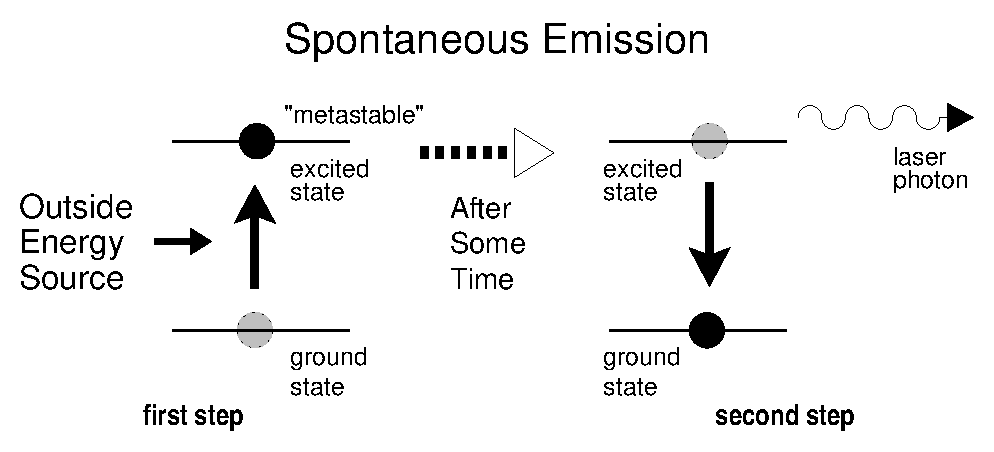
\includegraphics[width=5.in]{../../epsimages/laser-spontaneous_2.eps}
\end{center}
\caption{Spontaneous emission is a two step process, as shown here.  First, energy from an external source is applied to an atom in the laser medium, raising its energy to an excited (metastable) state.  After some time, it will decay back down to its ground state and emit the excess energy in the form of a photon.  This is the first stage in the formation of a laser beam. }
\label{laserse}
\end{figure}

\begin{figure}[!h]
\begin{center}
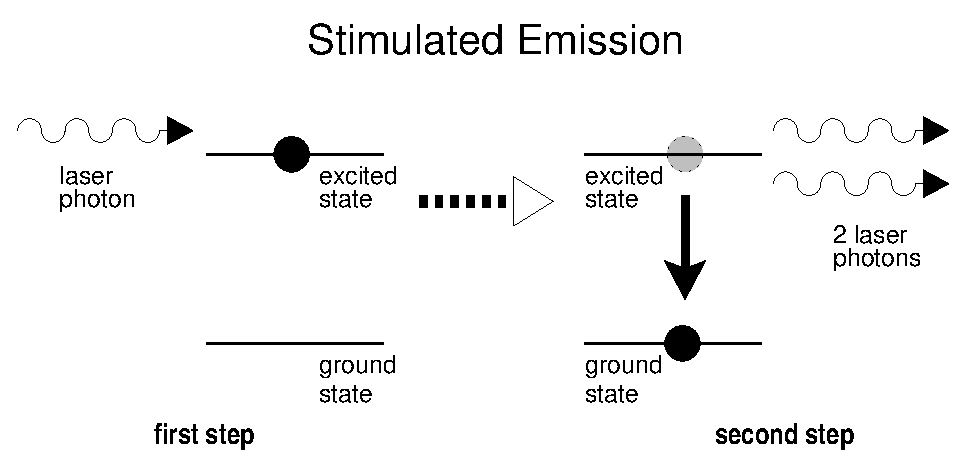
\includegraphics[width=5.in]{../../epsimages/laser-amplification_2.eps}
\end{center}
\caption{Stimulated emission is also a two step process, as shown here.  First, a laser photon encounters an atom that has been raised to an excited state, just like in the case of spontaneous emission.  The photon then causes the atom to decay to its ground state and emit another photon identical to the incoming photon.  This is the second step in the creation of a laser beam.  It happens many, many times as the laser photons pass through the optical cavity until the laser beam builds up to full strength.}
\label{laseramp}
\end{figure}


This can only happen if there are many electrons in a metastable state. If most of the electrons are in the ground state, then they will just \textit{absorb} the photons and no extra photons will be emitted. However, if more electrons are in the excited metastable state than in the ground state, then the process of stimulated emission will be able to continue. Usually in atoms, most of the electrons are in the lower energy levels and only a few are in excited states. When most of the electrons are in the excited metastable state and only a few are in the ground state, this is called \textbf{population inversion} (the populations in the excited and ground states are \textit{swapped} around) and this is when stimulated emission can occur. To start off the process, the electrons first have to be excited up into the metastable state. This is done using an external energy source.


\Definition{Population inversion}{Population inversion is when more atoms are in an excited state than in their ground state. It is a necessary condition to sustain a laser beam, so that there are enough excited atoms that can be stimulated to emit more photons.}


\begin{center}
\scalebox{1} % Change this value to rescale the drawing.
{
\begin{pspicture}(0,-1.46)(10.32,1.46)
\psline[linewidth=0.04cm](1.6,1.2)(4.42,1.2)
\psline[linewidth=0.04cm](1.6,-0.16)(4.42,-0.16)
\rput(0.77,-0.14){\footnotesize ground state}
\rput(0.76,1.3){\footnotesize metastable}
\rput(0.76,1.02){\footnotesize state}
\psline[linewidth=0.04cm](6.68,1.2)(9.5,1.2)
\psline[linewidth=0.04cm](6.68,-0.16)(9.5,-0.16)
\rput(5.85,-0.14){\footnotesize ground state}
\rput(5.84,1.3){\footnotesize metastable}
\rput(5.84,1.02){\footnotesize state}
\psdots[dotsize=0.12](2.16,-0.16)
\psdots[dotsize=0.12](2.36,-0.16)
\psdots[dotsize=0.12](2.58,-0.16)
\psdots[dotsize=0.12](2.8,-0.16)
\psdots[dotsize=0.12](3.02,-0.16)
\psdots[dotsize=0.12](3.24,-0.16)
\psdots[dotsize=0.12](3.46,-0.16)
\psdots[dotsize=0.12](3.66,-0.16)
\psdots[dotsize=0.12](7.26,1.18)
\psdots[dotsize=0.12](7.46,1.18)
\psdots[dotsize=0.12](7.68,1.18)
\psdots[dotsize=0.12](7.9,1.18)
\psdots[dotsize=0.12](8.12,1.18)
\psdots[dotsize=0.12](8.34,1.18)
\psdots[dotsize=0.12](8.56,1.18)
\psdots[dotsize=0.12](8.76,1.18)
\psdots[dotsize=0.12](2.68,1.18)
\psdots[dotsize=0.12](3.06,1.2)
\psdots[dotsize=0.12](3.46,1.18)
\psdots[dotsize=0.12](7.6,-0.18)
\psdots[dotsize=0.12](7.98,-0.16)
\psdots[dotsize=0.12](8.38,-0.18)
\rput(2.1,-0.915){usually most electrons are in }
\rput(7.65,-0.895){most electrons in excited metastable}
\rput(7.66,-1.235){state = \textit{population inversion}}
\rput(1.18,-1.215){the ground state}
\end{pspicture} 
}
\end{center}

Therefore, materials used to make laser light \textit{must} must have metastable states which can allow population inversion to occur when an external energy source is applied. Some substances which are used to make lasers are listed in table~\ref{lasertypes}. You can see that gases (such as Helium-Neon mixture), liquids (such as dyes), and solids (such as the precious stone ruby) are all used to make lasers. 


\begin{table}[H]
\begin{center}
\begin{tabular}{p{3cm}ccp{3cm}}
\hline
\textbf{Material} & \textbf{Type} & \textbf{Wavelength} & \textbf{Uses} \\
\hline
Helium--Neon & gas & 632,8 nm & scientific research, holography \\
%Argon ion & gas & 488.0 nm, 514.5 nm & medicine, \\
%Carbon dioxide & gas & 10.6 $\mu$m, 9.4 $\mu$m & industry (cutting, welding), surgery \\
%Helium--Cadmium & vapor & 440 nm, 325 nm & printing, scientific research \\
Argon ion & gas & 488,0 nm & medicine \\
Carbon dioxide & gas & 10,6 $\mu$m & industry (cutting, welding), surgery \\
Helium--Cadmium & vapour & 325 nm & printing, scientific research \\
Ruby & solid--state & 694,3 nm & holography \\
Neodymium YAG (Yttrium Aluminium Garnet) & solid--state & 1,064 $\mu$m & industry, surgery, research \\
Titanium--Sapphire & solid--state & 650--1100 nm & research \\
Laser diode & semiconductor & 375--1080 nm & telecommunications, industry, printing, CD players, laser pointers \\
\hline
\end{tabular}
\end{center}
\caption{A selection of different lasers. The laser material and general type of each laser is given, along with typical wavelengths of the laser light they create. Examples of real-world applications are also given. All these materials allow a population inversion to be set up.}
\label{lasertypes}
\end{table}


%\begin{IFact}
%{The first working laser, using synthetic ruby as the laser material, was made by Theodore H. Maiman at Hughes Research Laboratories in Malibu, California. Later in the same year the Iranian physicist Ali Javan, together with William Bennet and Donald Herriot, made the first gas laser using helium and neon. Javan received the Albert Einstein Award in 1993.}
%\end{IFact}


\subsection{A simple laser}


A laser consists of a number of different parts that work together to create the laser beam.  Figure~\ref{lasercavity} shows the different parts of the laser, while Figure~\ref{laserprocess} shows how they create the laser beam.\\

\begin{figure}[!htb]
\begin{center}
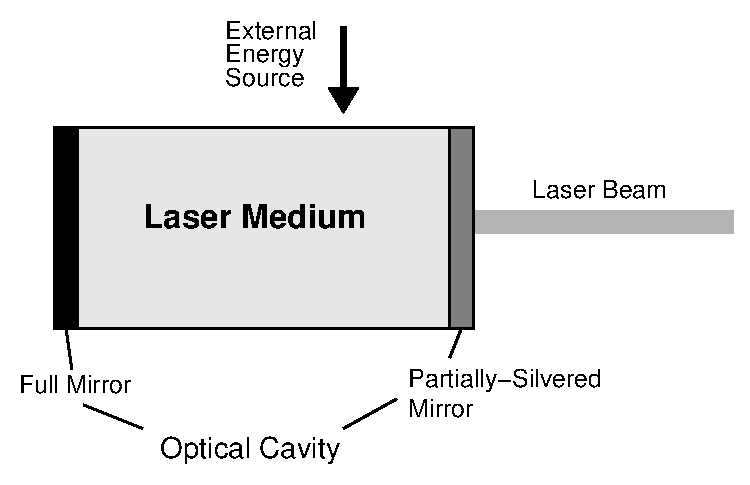
\includegraphics[width=4.8in]{../../epsimages/laser-cavity_2.eps}
\end{center}
\caption{Diagram of a laser showing the main components.}
\label{lasercavity}
\end{figure}


\begin{figure}[!tb]
\begin{center}
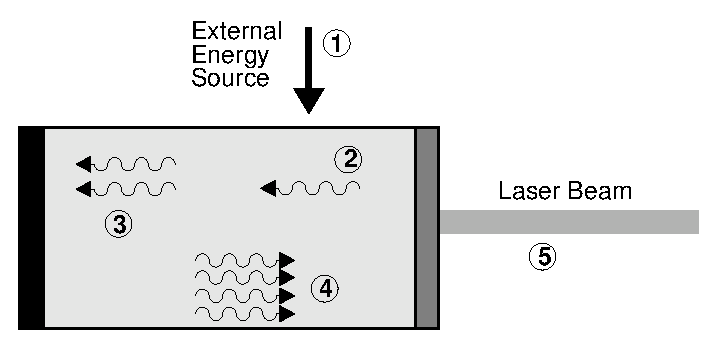
\includegraphics[width=4.5in]{../../epsimages/laser-process.eps}
\end{center}
\caption{Diagram of a laser showing the process of creating a laser beam. (1) A source of external energy is applied to the laser medium, raising the atoms to an excited state. (2) An excited atom decays though spontaneous emission, emitting a photon.  (3) The photon encounters another excited atom and causes it to decay through stimulated emission, creating another photon. (4) The photons bounce back and forth through the laser medium between the mirrors, building up more and more photons.  (5) A small percentage of the photons pass through the partially-silvered mirror to become the laser beam we see.}
\label{laserprocess}
\end{figure}
 
The basis of the laser is the laser material which consists of the atoms that are used to create the laser beam. Many different materials can be used as laser material, and their energy levels determine the characteristics of the laser. Some examples of different lasers are shown in Table~\ref{lasertypes}. The laser material is contained in the optical cavity.\\ 
 
Before the laser is turned on, all the atoms in the laser material are in their ground state. The first step in creating a laser beam is to add energy to the laser material to raise most of the electrons into an excited metastable state. This is called \textit{pumping} the laser. \\ 

The creation of the laser beam starts through the process of \textit{spontaneous emission}, shown in Figure~\ref{laserse}. An electron drops down to the ground state and emits a photon with energy equal to the energy difference of the two energy levels. This laser photon is the beginning of the laser beam.\\

At some time a laser photon will run into another excited electron. Then stimulated emission occurs and the electron drops down to the ground state and emits an additional identical photon as shown in Figure~\ref{laseramp}. Since the laser material typically has a large number of atoms, one laser photon passing through this material will rapidly cause a large number of photons just like it to be emitted.
 
The optical cavity keeps the laser photons inside the laser cavity so that they can build up the laser beam. At each end is a concave mirror; one is a full mirror and one is a partial mirror. The full mirror is totally reflective. The partial mirror transmits a small amount of the light that hits it (less than 1\%). The mirrors are carefully aligned so that photons that reflect off one mirror become ``trapped'', and bounce back and forth between the mirrors many times causing more and more stimulated emission. The photons that eventually escape through the partially-silvered mirror become the laser beam that we see.
 
\begin{IFact}
{In 1953, Charles Townes and graduate students James Gordon and
  Herbert Zeiger produced the first maser, a device operating on
  similar principles to the laser, but producing microwave rather than
  optical radiation. Townes's maser could not make a continuous
  beam. Nikolay Basov and Aleksandr Prokhorov of the former Soviet
  Union worked in\-dependently and developed a method of making a
  continuous beam using more than two energy levels. Townes, Basov and
  Prokhorov shared the Nobel Prize in Physics in 1964.}
\end{IFact}

As the photons bounce between mirrors, they continually pass through the laser material, stimulating those atoms to emit more photons.  This creates an ever increasing beam of photons, all with the same characteristics, all travelling in the same direction.  In this way, the optical cavity helps to amplify the original laser photons into a concentrated, intense beam of photons.

The laser cavity also helps to narrow the frequency range of laser light emitted. The distance between the two mirrors defines the cavity \textit{mode} which only allows light of a narrow range of frequencies to continue being reflected back and forth. Light of other frequencies damped out. (This is just like in the chapter on the physics of music where a pipe of a certain length corresponds to a particular wavelength of sound.) Therefore only a narrow frequency of light can be emitted.


\subsection{Laser applications and safety}
Although the first working laser was only produced in 1958, lasers are now found in many household items. For example, lasers are well-known through their use as cheap laser pointers. However, lasers can be very dangerous to the human eye since a large amount of energy is focused into a very narrow beam. \textbf{NEVER POINT A LASER POINTER INTO SOMEBODY'S EYES - IT CAN BLIND THEM FOREVER.}

Other uses include:
\begin{itemize}
\item Semiconductor lasers which are small, efficient and cheap to make are used in CD players. 
\item He-Ne Lasers are used in most grocery shops to read in the price of items using their barcodes. This makes the cashiers' job much quicker and easier.
\item High energy lasers are used in medicine as a cutting and welding tool. Eye surgery in particular make use of the precision of lasers to reattach the retinas of patients' eyes. The heat from cutting lasers also helps to stop the bleeding of a wound by burning the edges (called cauterising).
\end{itemize}
% PhET simulation on lasers: SIYAVULA-SIMULATION:http://cnx.org/content/m39557/latest/#id6348

\simulation{Lasers}{Vpqof}

\clearpage

\Activity{Case Study}{Uses of lasers}
{
Do research in a library or on the Internet on one application of laser technology. Explain how the technology works by using a laser.\\
You will need to present your findings to the class in the form of a poster. You can think of any useful application, but to give you some ideas of where to start, some applications are listed below:
\begin{itemize}
\item laser printers
\item laser communication and fibre optics
\item optical storage
\item using lasers as precision measurement tools
\item your own ideas...
\end{itemize}
}


\Exercise{Lasers}{
\begin{enumerate}
\item Explain what is meant by \textit{spontaneous emission of radiation}.
\item Explain what is meant by \textit{stimulated emission of radiation}.
\item List the similarities and differences between spontaneous emission of radiation and stimulated emission of radiation.
\item How is the light emitted by a laser different from the light emitted by a light bulb?
\item Describe using a simple diagram, how a laser works. Your description should include the following concepts: metastable state and population inversion.
\item Give examples of some materials that have been used for lasers. What do all these materials have in common? 
\item Describe how the laser cavity affects:
\begin{itemize}
\item increasing amplification
\item concentrating beam intensity
\item narrowing the frequency of the beam
\end{itemize}
\item List some applications of lasers.
\end{enumerate}

% Automatically inserted shortcodes - number to insert 8
\par \practiceinfo
\par \begin{tabular}[h]{cccccc}
% Question 1
(1.)	01n1	&
% Question 2
(2.)	01n2	&
% Question 3
(3.)	01n3	&
% Question 4
(4.)	01n4	&
% Question 5
(5.)	01n5	&
% Question 6
(6.)	01n6	\\ % End row of shortcodes
% Question 7
(7.)	01n7	&
% Question 8
(8.)	01n8	&
\end{tabular}
% Automatically inserted shortcodes - number inserted 8

}
% Presentation on optical phenomena: SIYAVULA-PRESENTATION:http://cnx.org/content/m39557/latest/#slidesharefigure


\summary{VPqph}
\begin{itemize}
\item Light of the correct frequency can eject electrons from a metal. This is called the photoelectric effect.
\item A metal has a work function which is the minimum energy needed to emit an electron from the metal. 
\item Emission spectra are formed by glowing gases. The pattern of the spectra is characteristic of the specific gas. 
\item Absorption spectra are formed when certain frequencies of light are absorbed by a material.
\item Lasers are devices that produce a special type of light that has many uses.
\item Lasers have many uses,for example, in CD and DVD players, to cut material, in surgery, in printing, in telecommunications and as laser pointers.
\end{itemize}


\begin{eocexercises}{}
\begin{enumerate}
\item What is the photoelectric effect? 
\item Calculate the energy of a photon of red light with a wavelength of 400~nm.
\item Will ultraviolet light with a wavelength of 990~nm be able to emit electrons from a sheet of calcium with a work function of 2,9~eV?
\item What does the acronym LASER stand for?
\item Name three types of lasers and their uses.
\item Write a short essay on the benefits lasers have had on modern society.
\end{enumerate}

% Automatically inserted shortcodes - number to insert 6
\par \practiceinfo
\par \begin{tabular}[h]{cccccc}
% Question 1
(1.)	01n9	&
% Question 2
(2.)	01na	&
% Question 3
(3.)	01nb	&
% Question 4
(4.)	01nc	&
% Question 5
(5.)	01nd	&
% Question 6
(6.)	01ne	\\ % End row of shortcodes
\end{tabular}
% Automatically inserted shortcodes - number inserted 6
\end{eocexercises}
